\subsection{Diseño de vistas}

\subsubsection{Vista de inicio de sesión}

\begin{figure}[H]
    \centering
    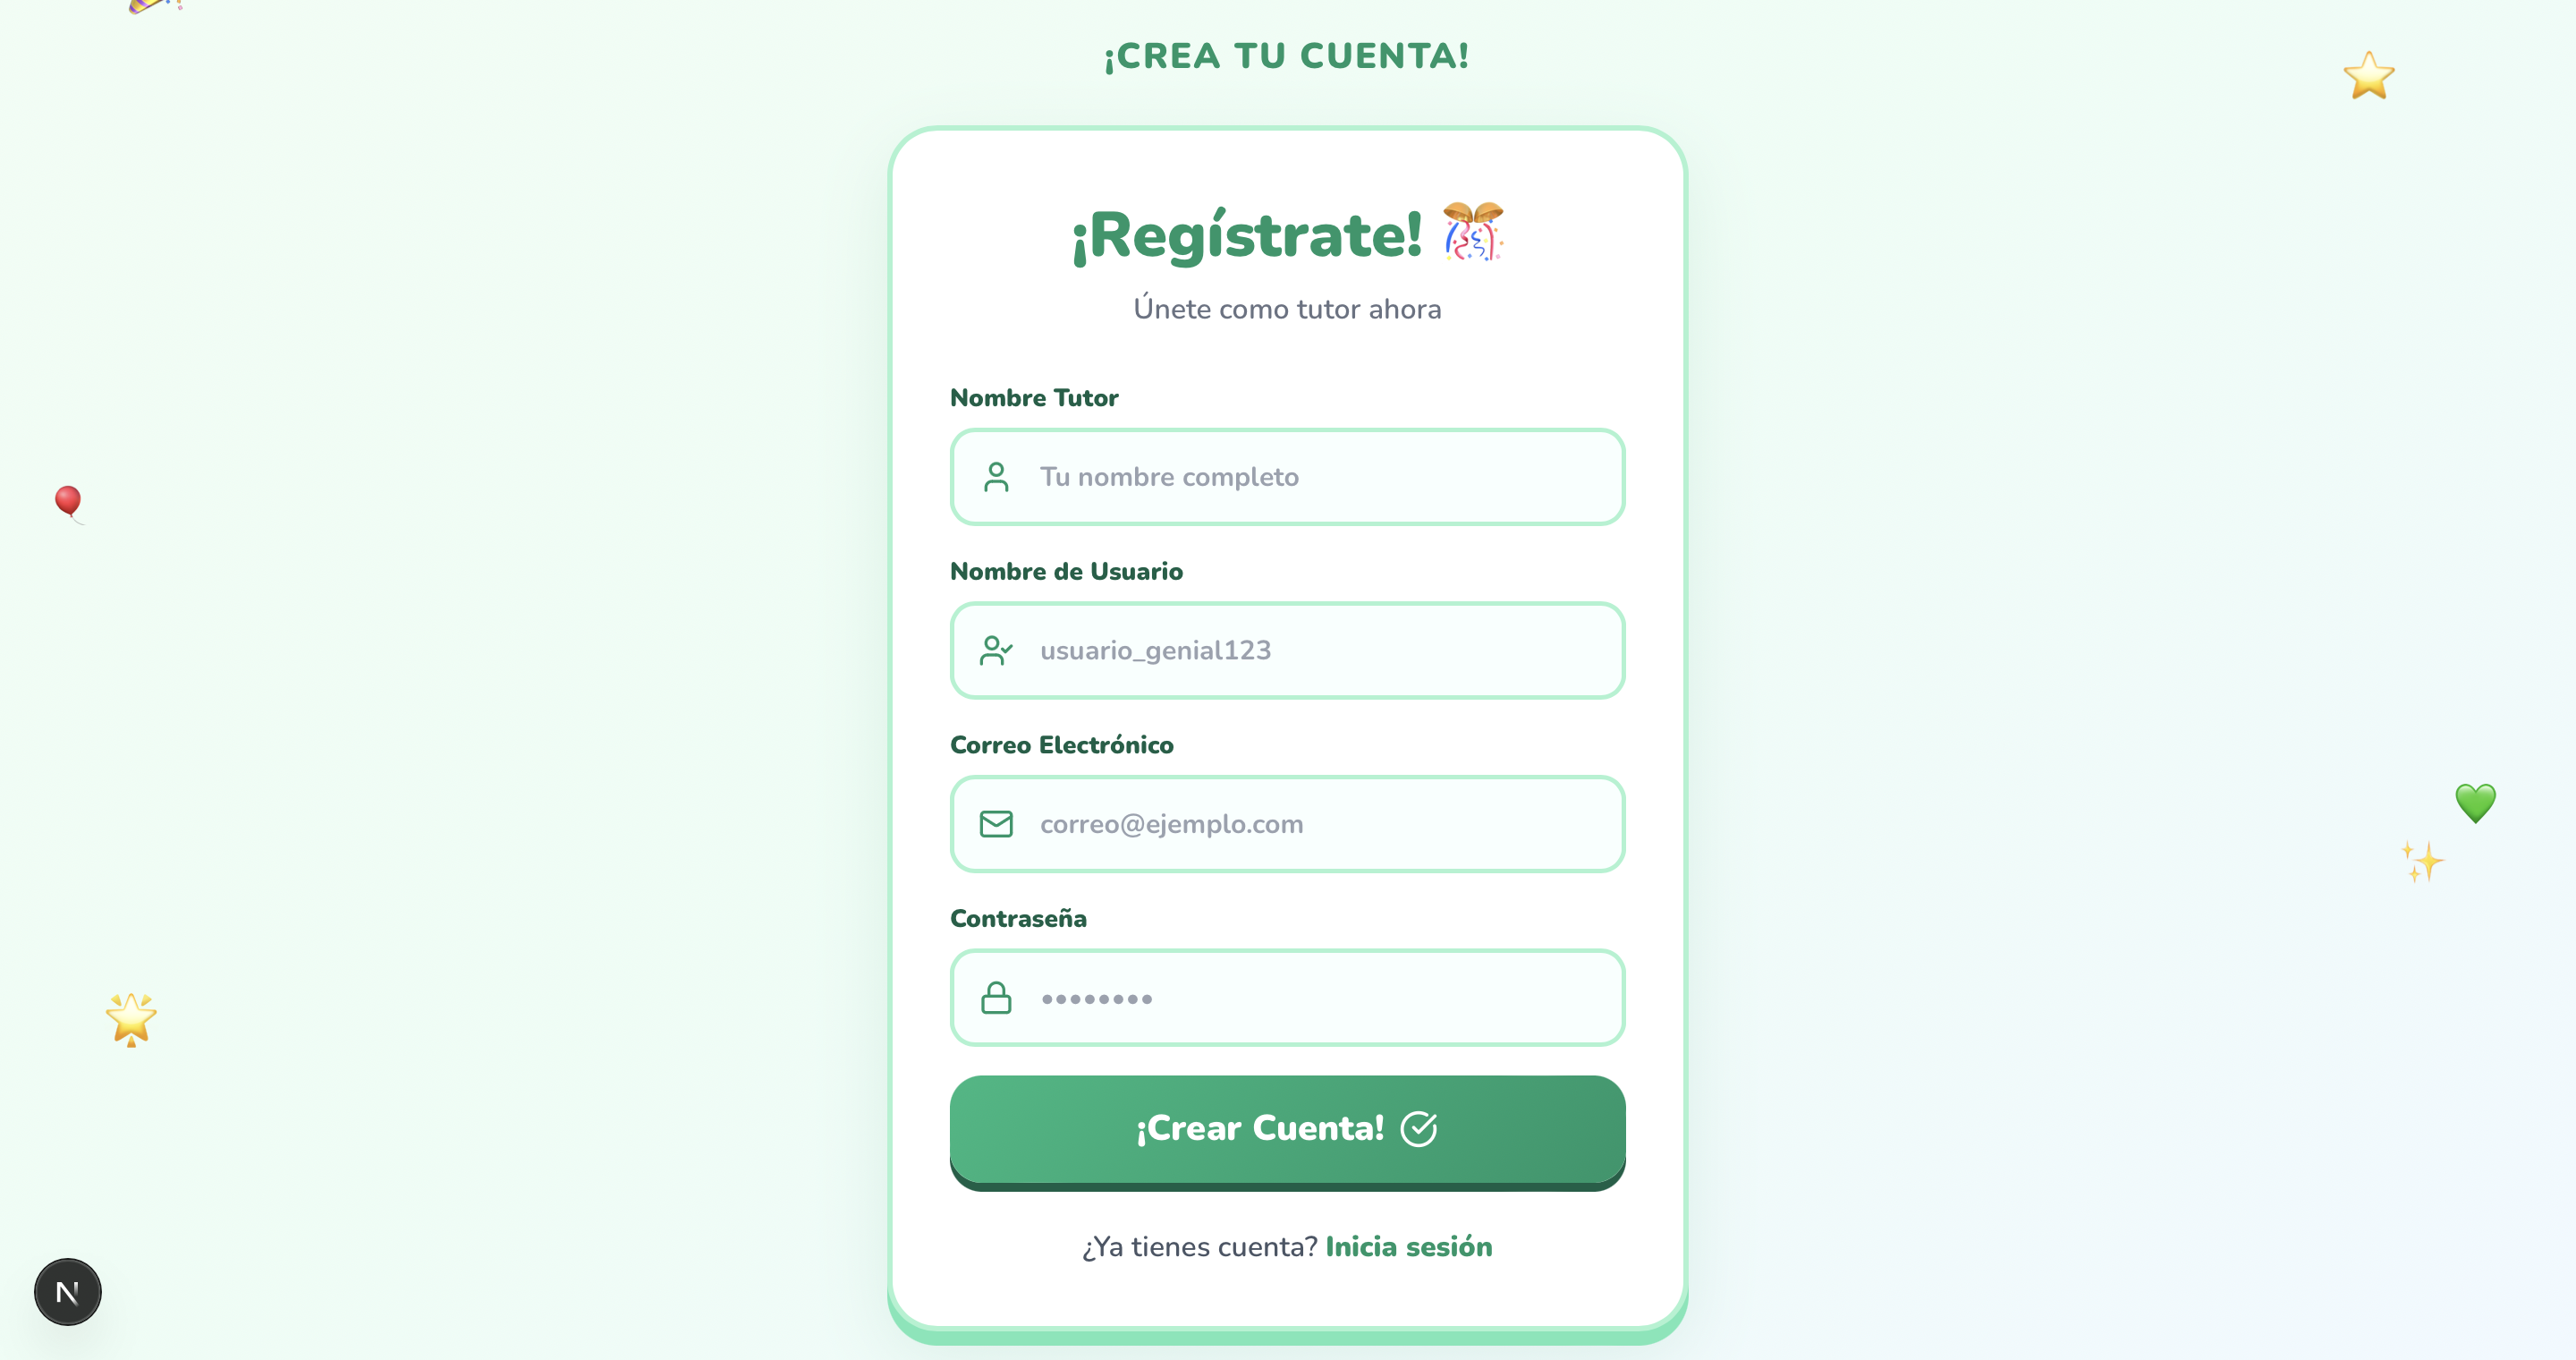
\includegraphics[width=0.7\textwidth]{Imagenes/registrar.png}
    \caption{Registro de nuevo usuario}
    \label{fig:registrar}
\end{figure}

\begin{figure}[H]
    \centering
    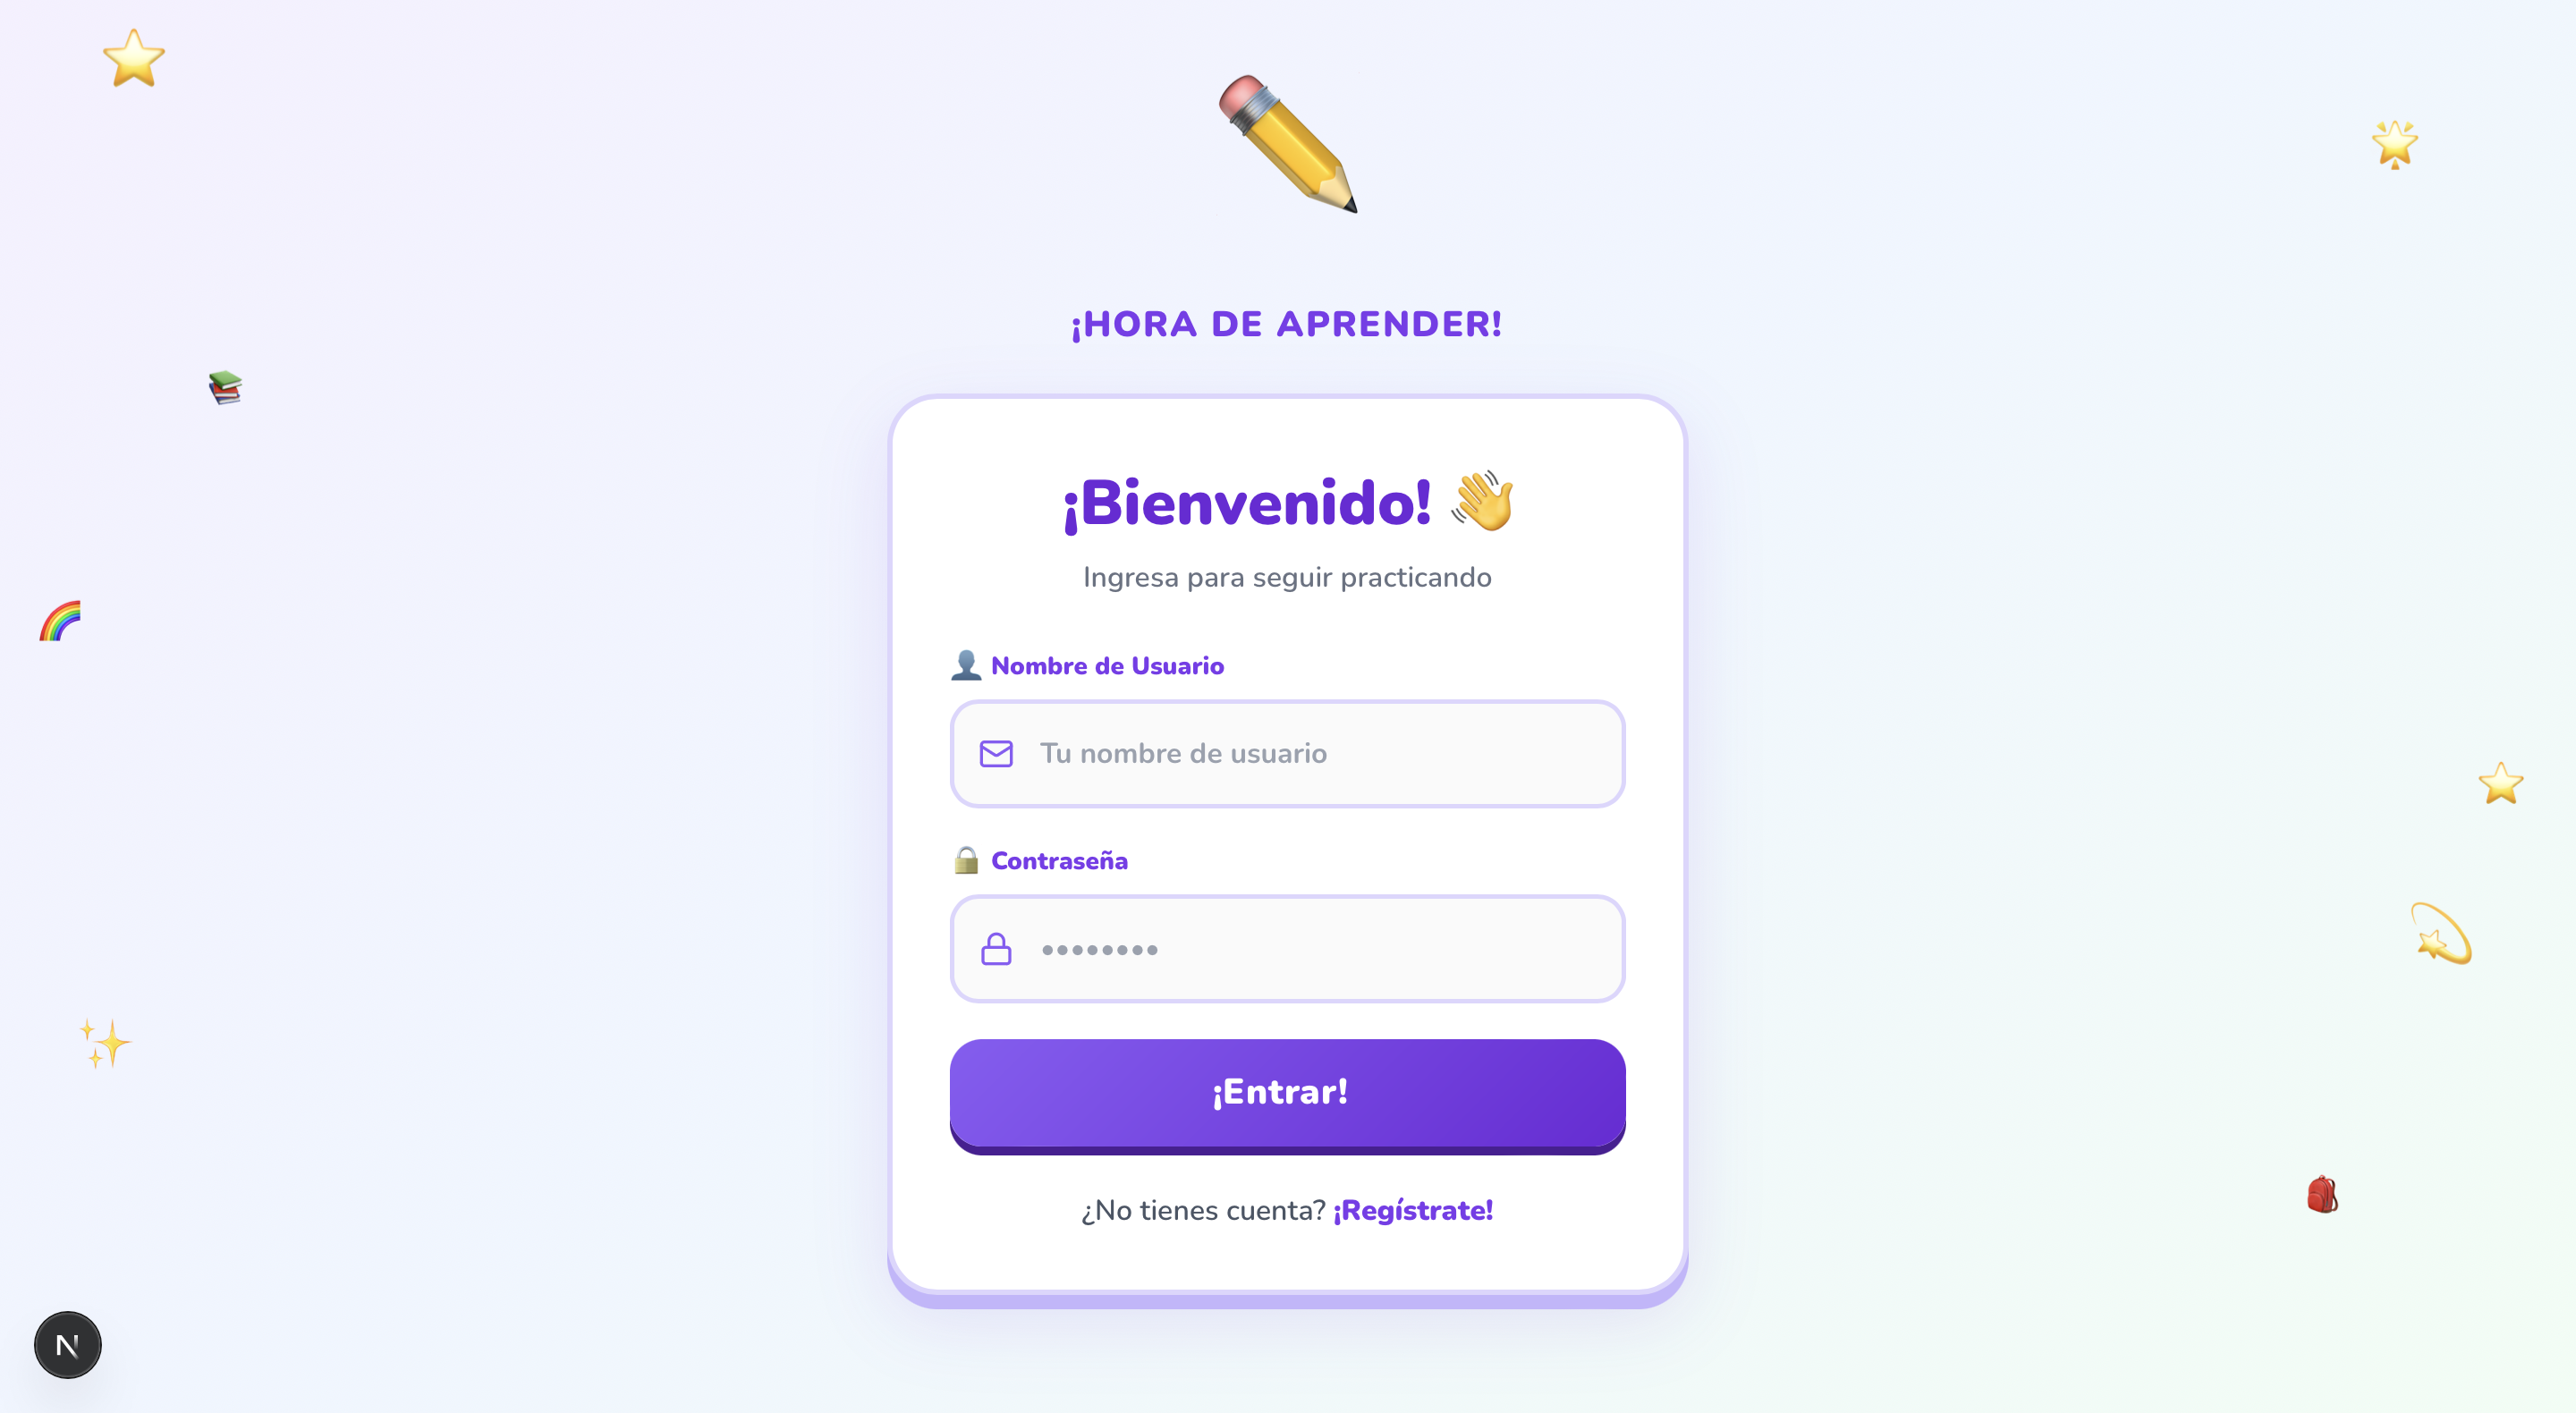
\includegraphics[width=0.7\textwidth]{Imagenes/login.png}
    \caption{Inicio de sesión}
    \label{fig:login}
\end{figure}

\subsubsection{Vistas del tutor}

\begin{figure}[H]
    \centering
    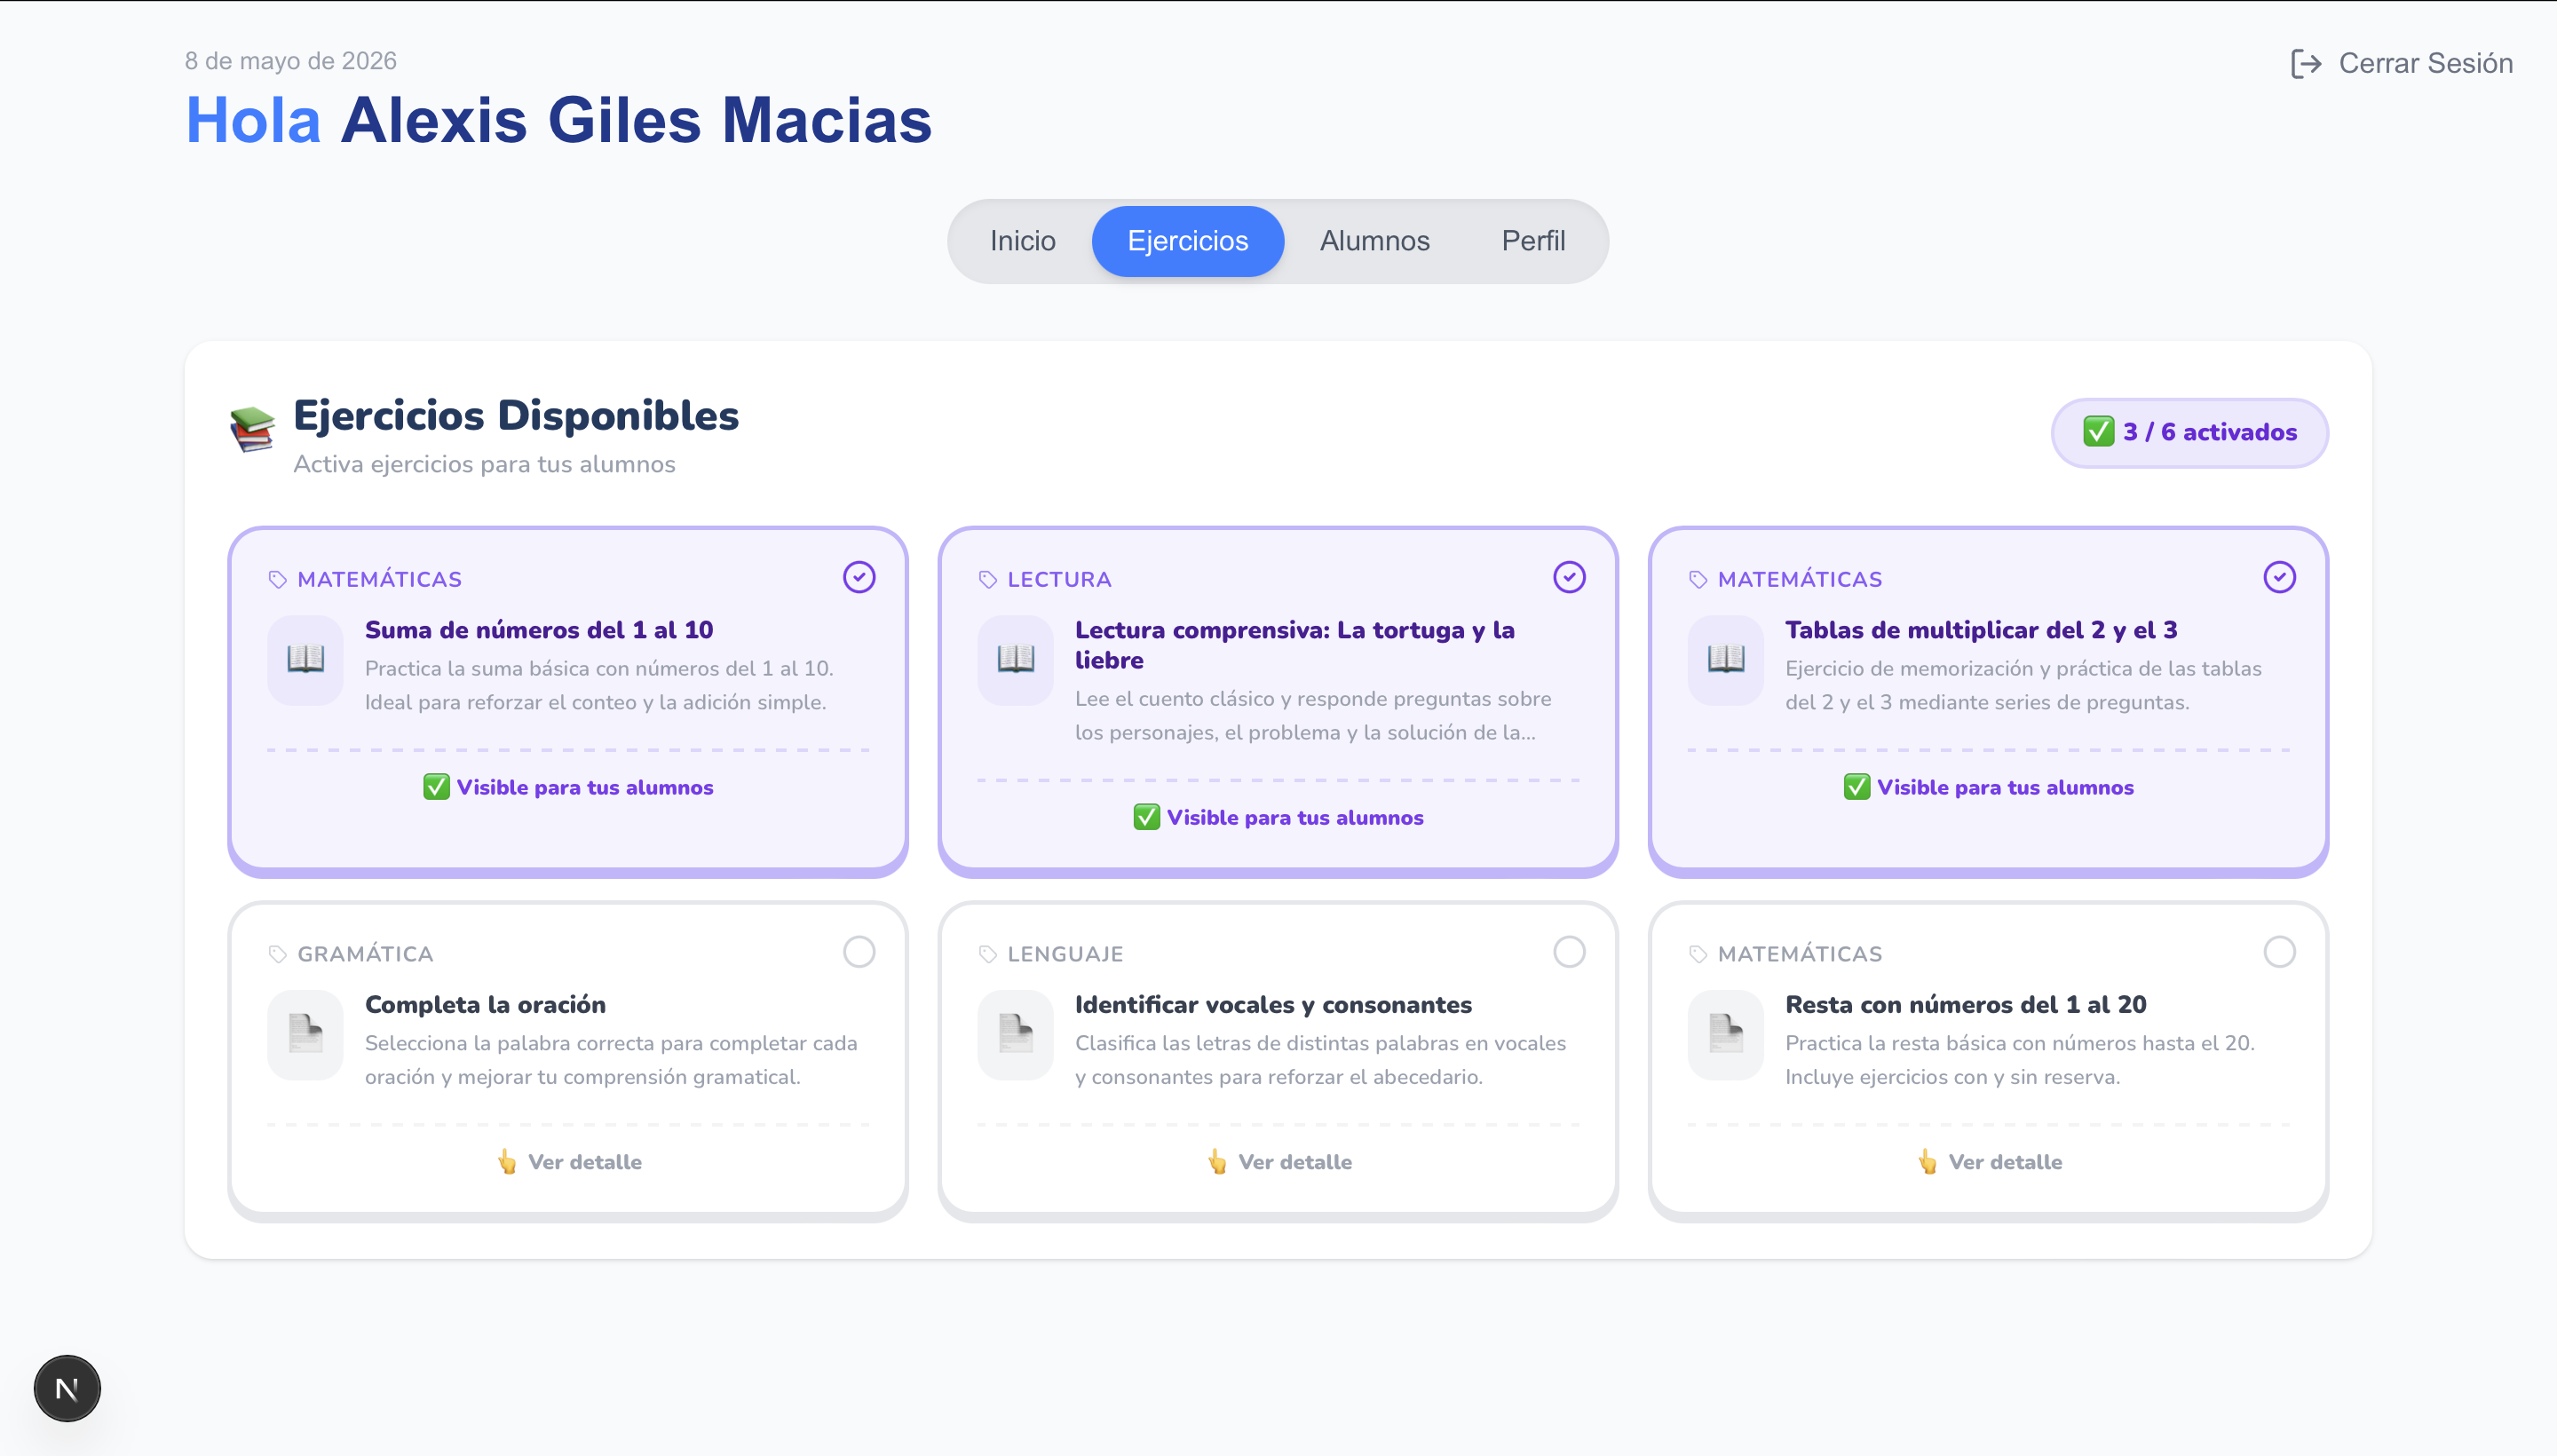
\includegraphics[width=0.7\textwidth]{Imagenes/EjerciciosTutor.png}
    \caption{Catalogo de ejercicios para tutor y ejercicios}
    \label{fig:ejeTu}
\end{figure}

\begin{figure}[H]
    \centering
    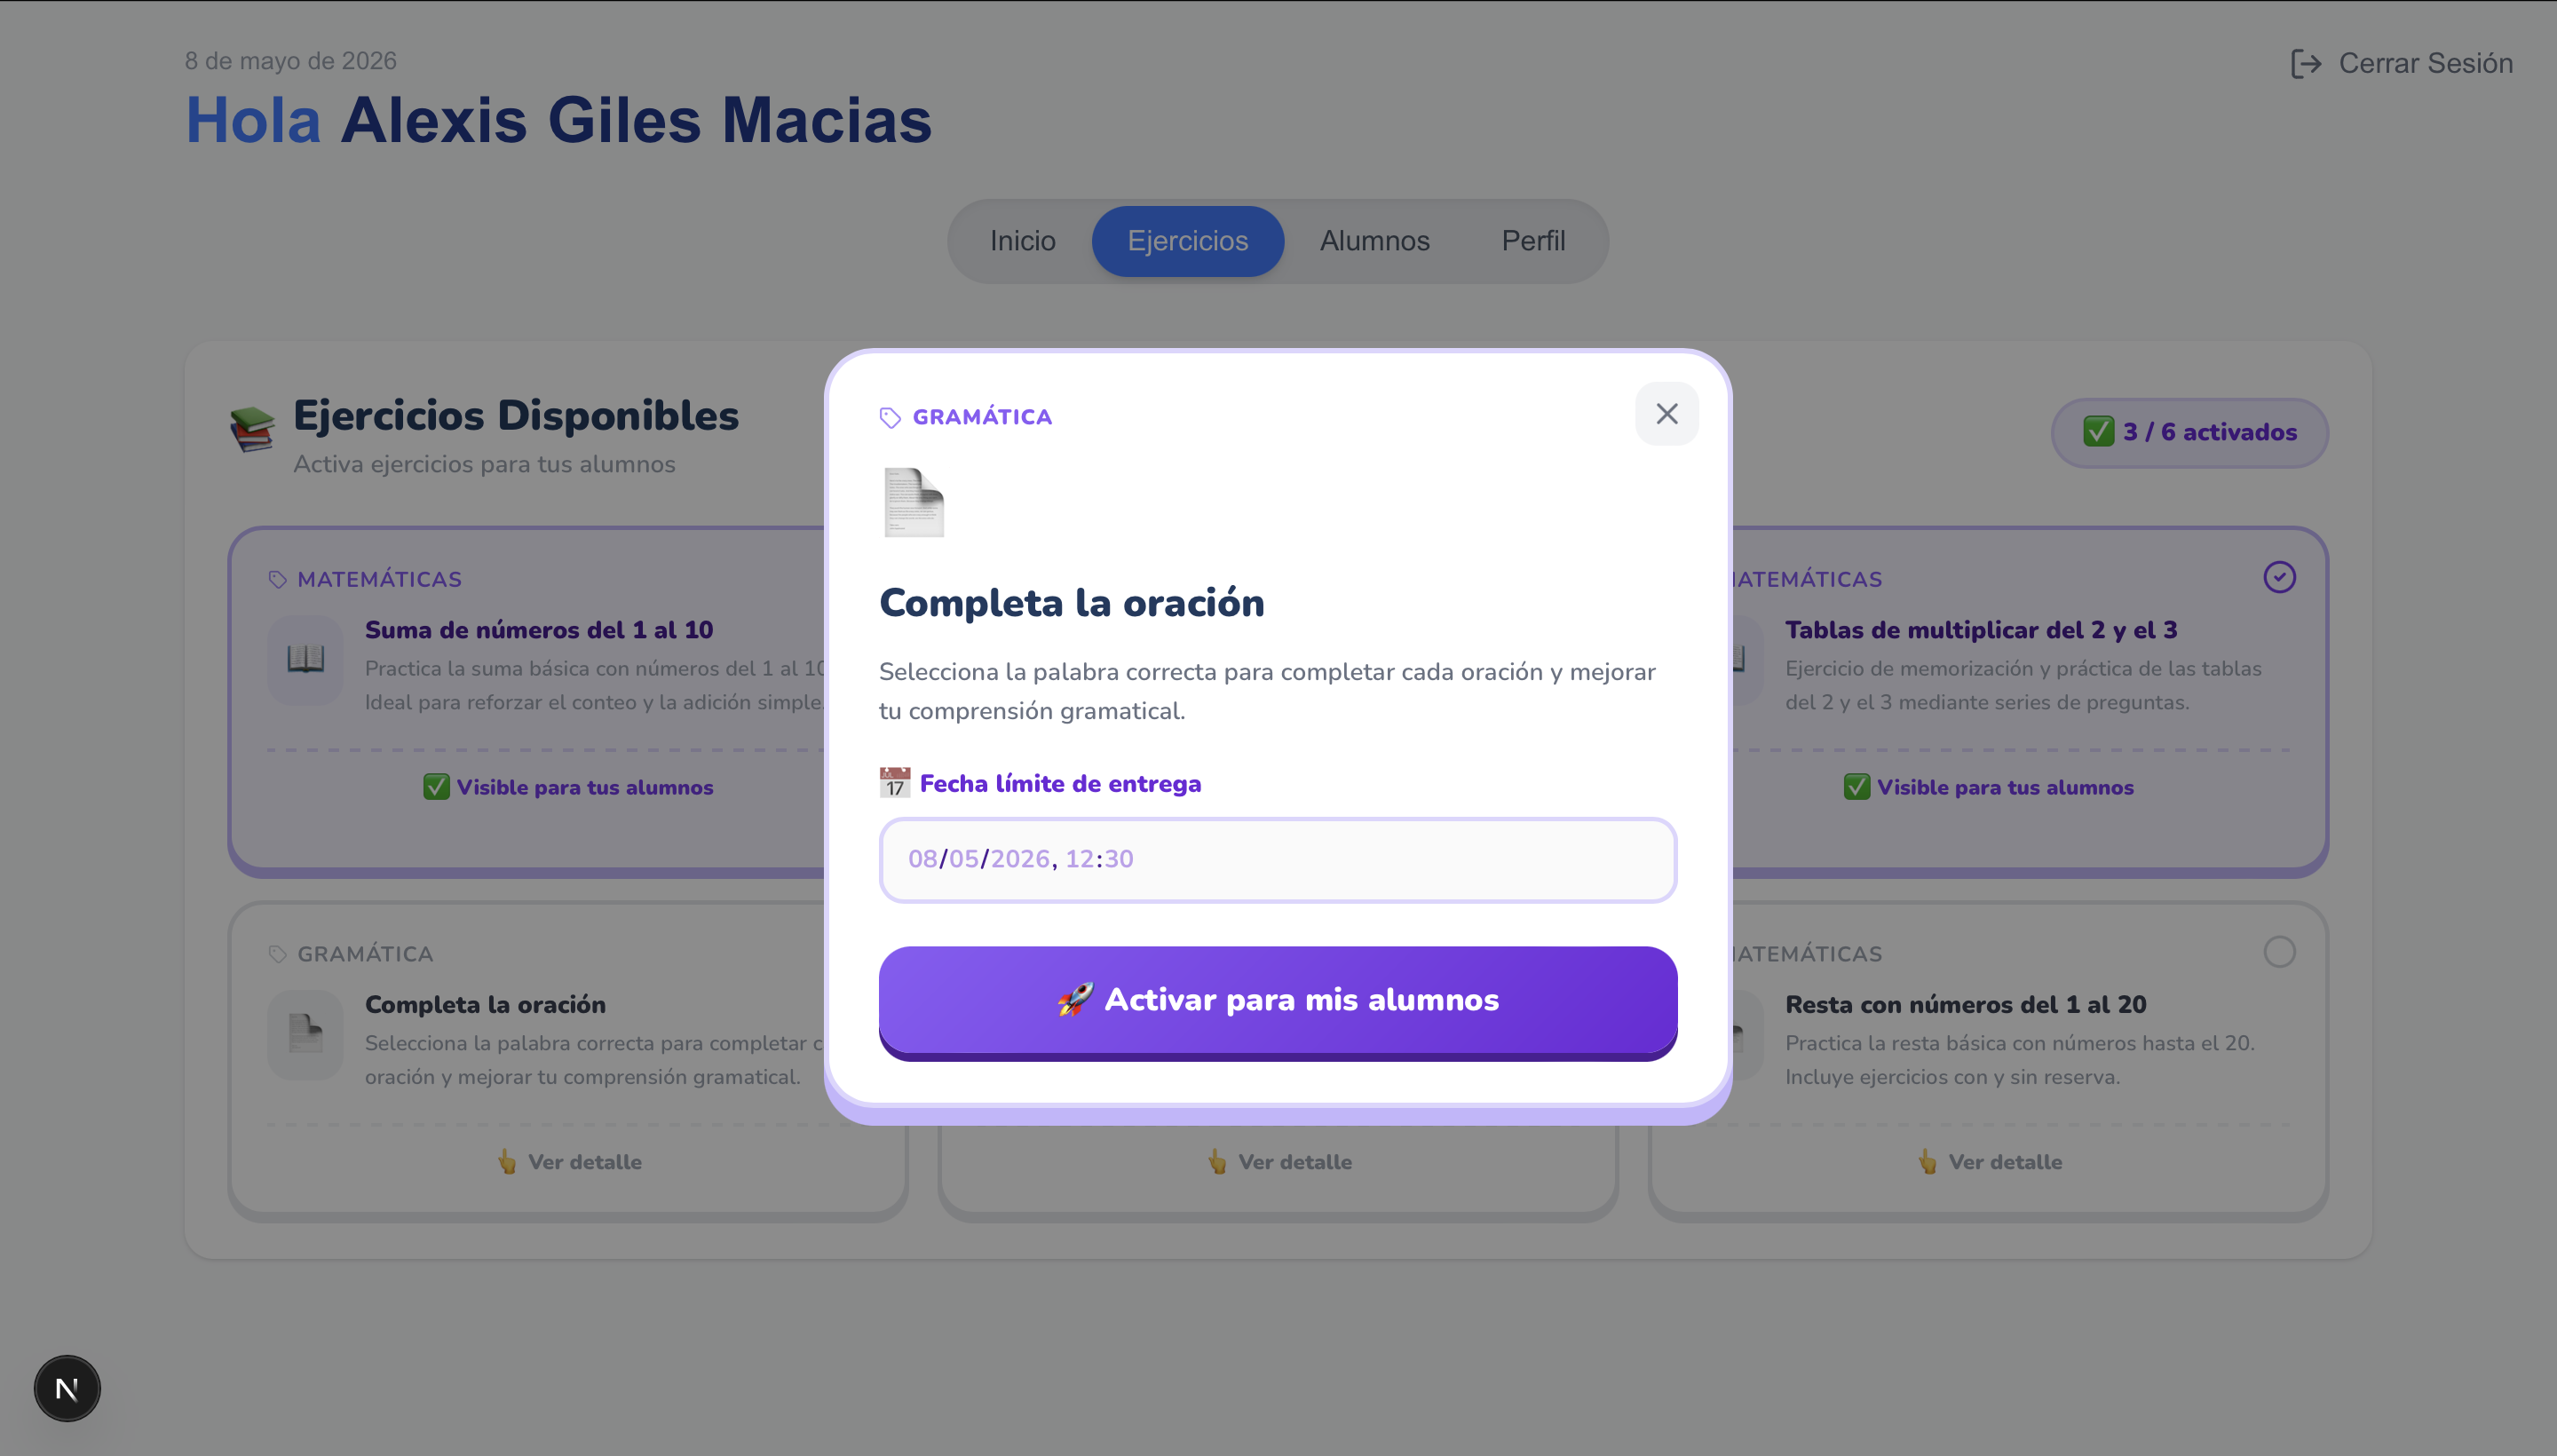
\includegraphics[width=0.7\textwidth]{Imagenes/asignacion.png}
    \caption{Asignacion de ejercicios a alumnos}
    \label{fig:asignacionEje}
\end{figure}

\begin{figure}[H]
    \centering
    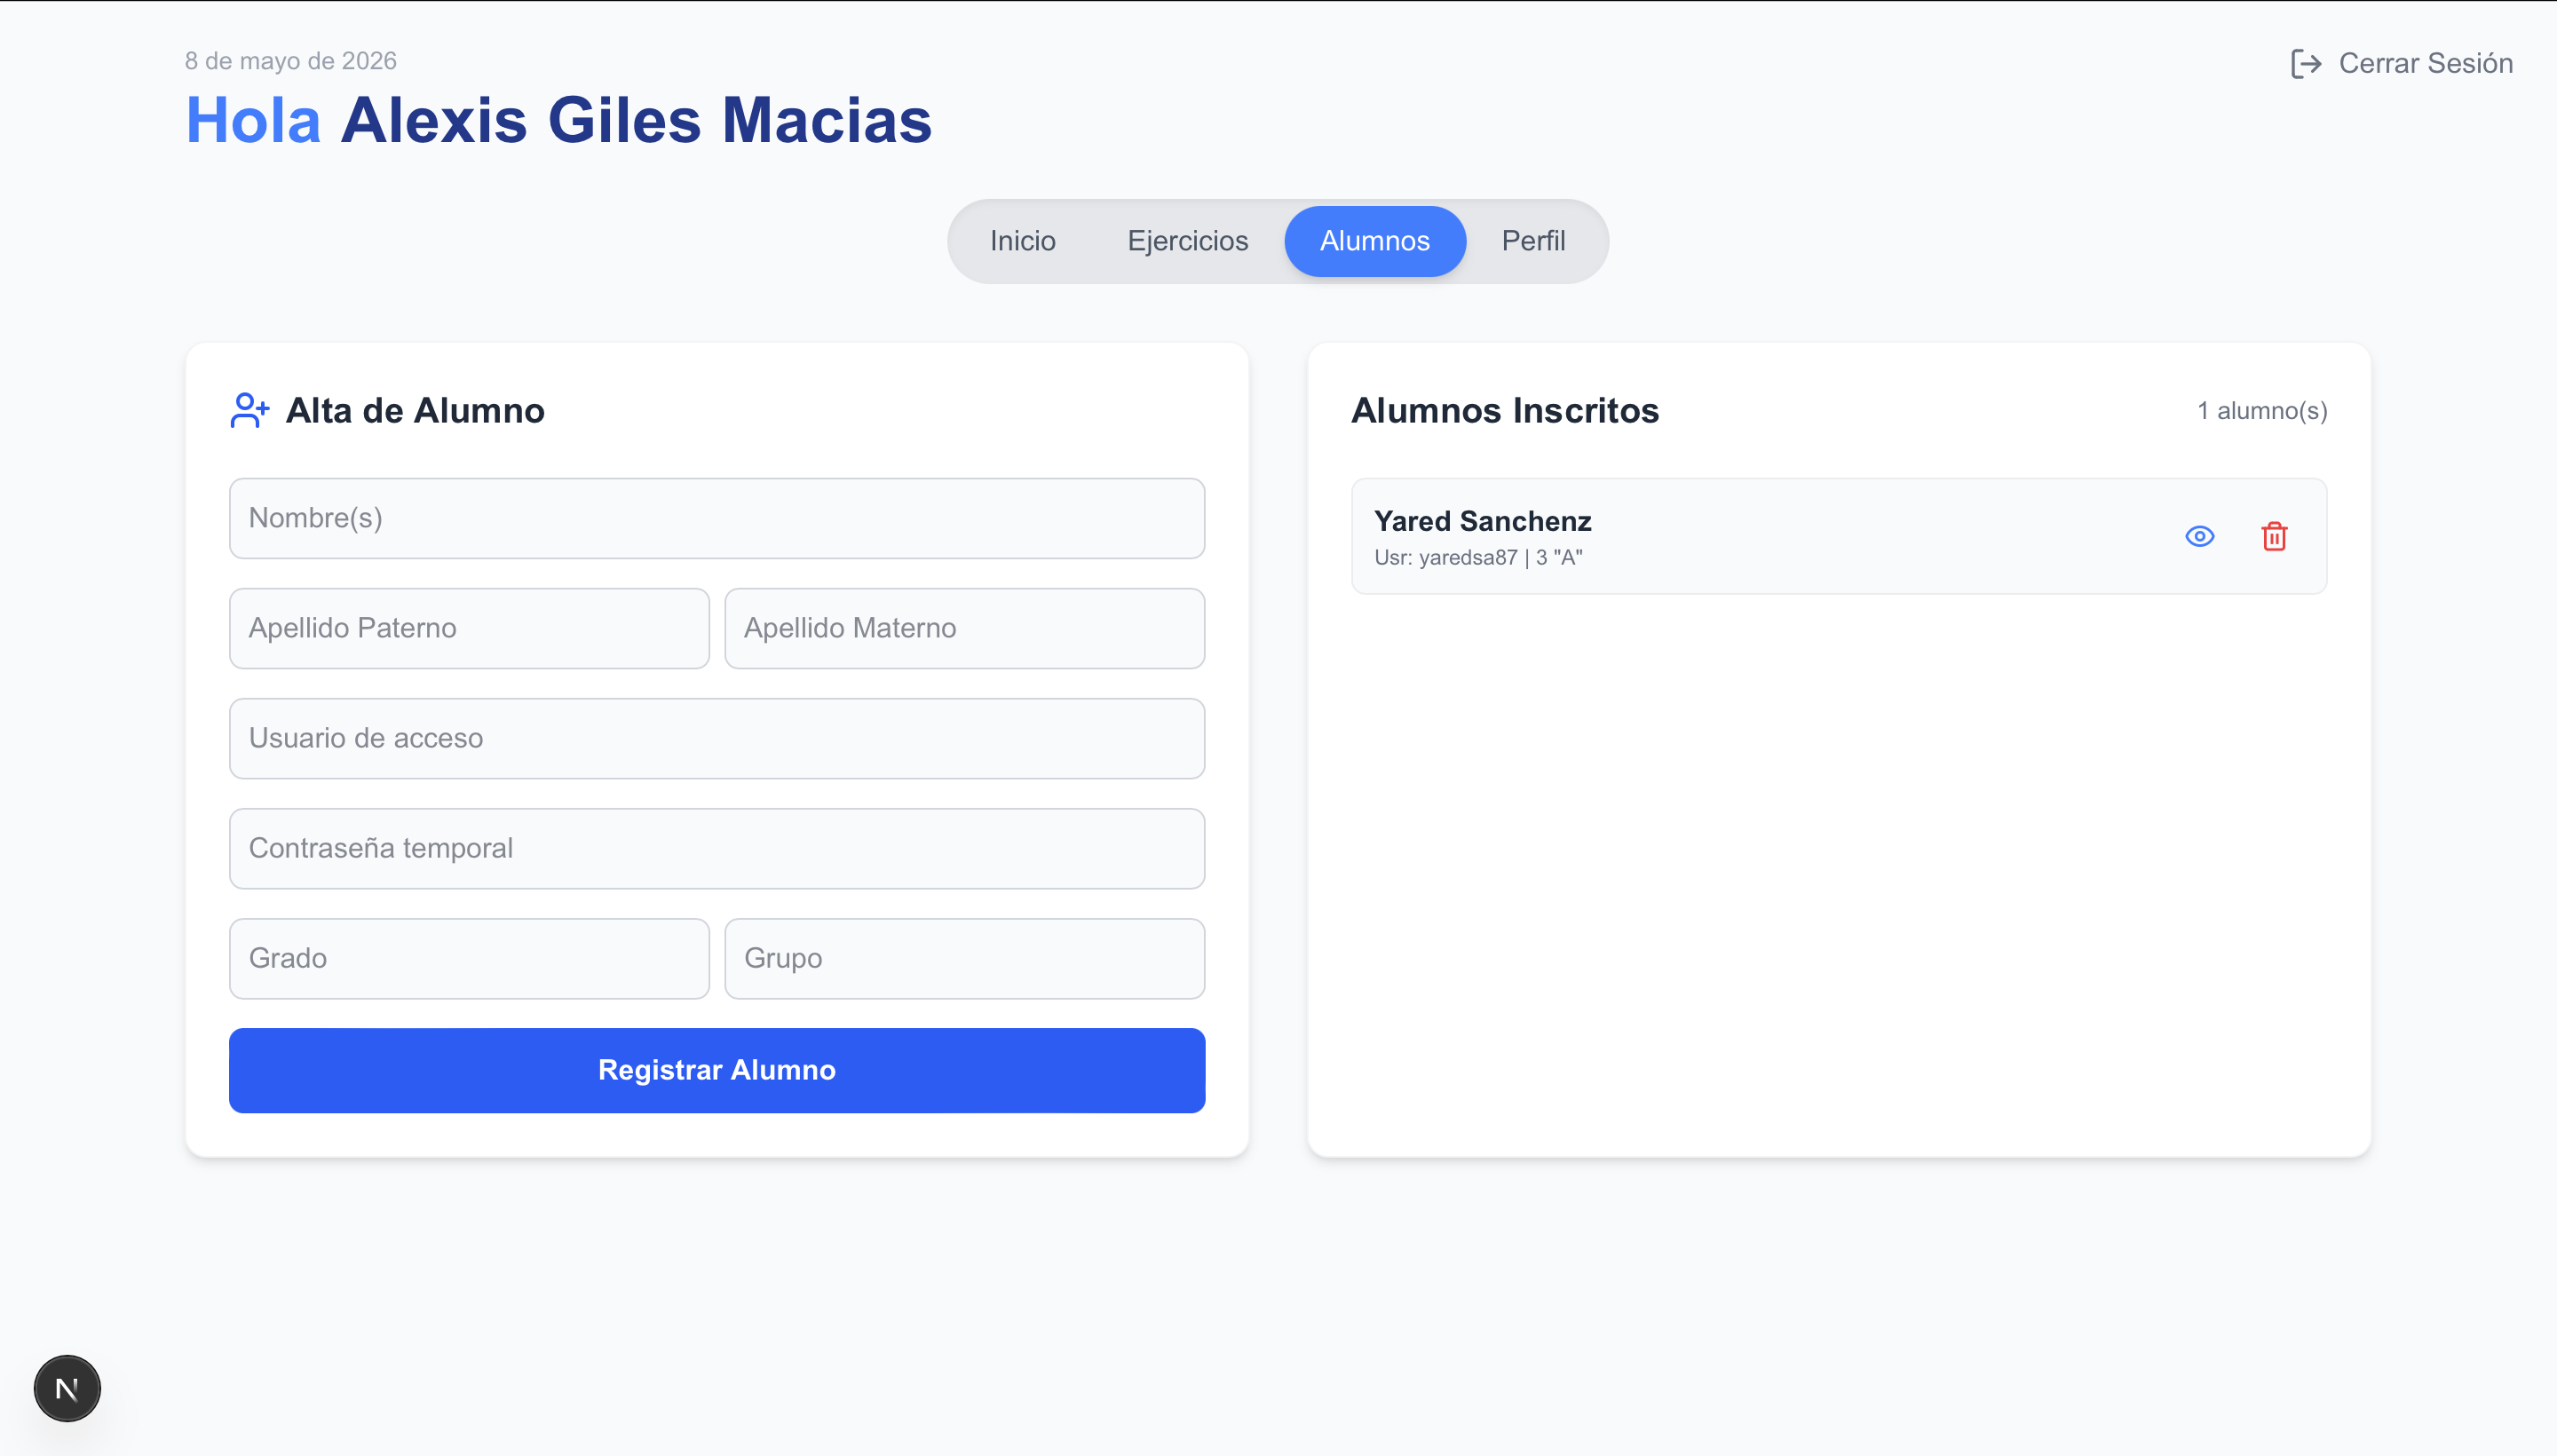
\includegraphics[width=0.7\textwidth]{Imagenes/AlumnosInscritos.png}
    \caption{Alta de alumnos y visualización de alumnos inscritos}
    \label{fig:alumnosInscritos}
\end{figure}

\begin{figure}[H]
    \centering
    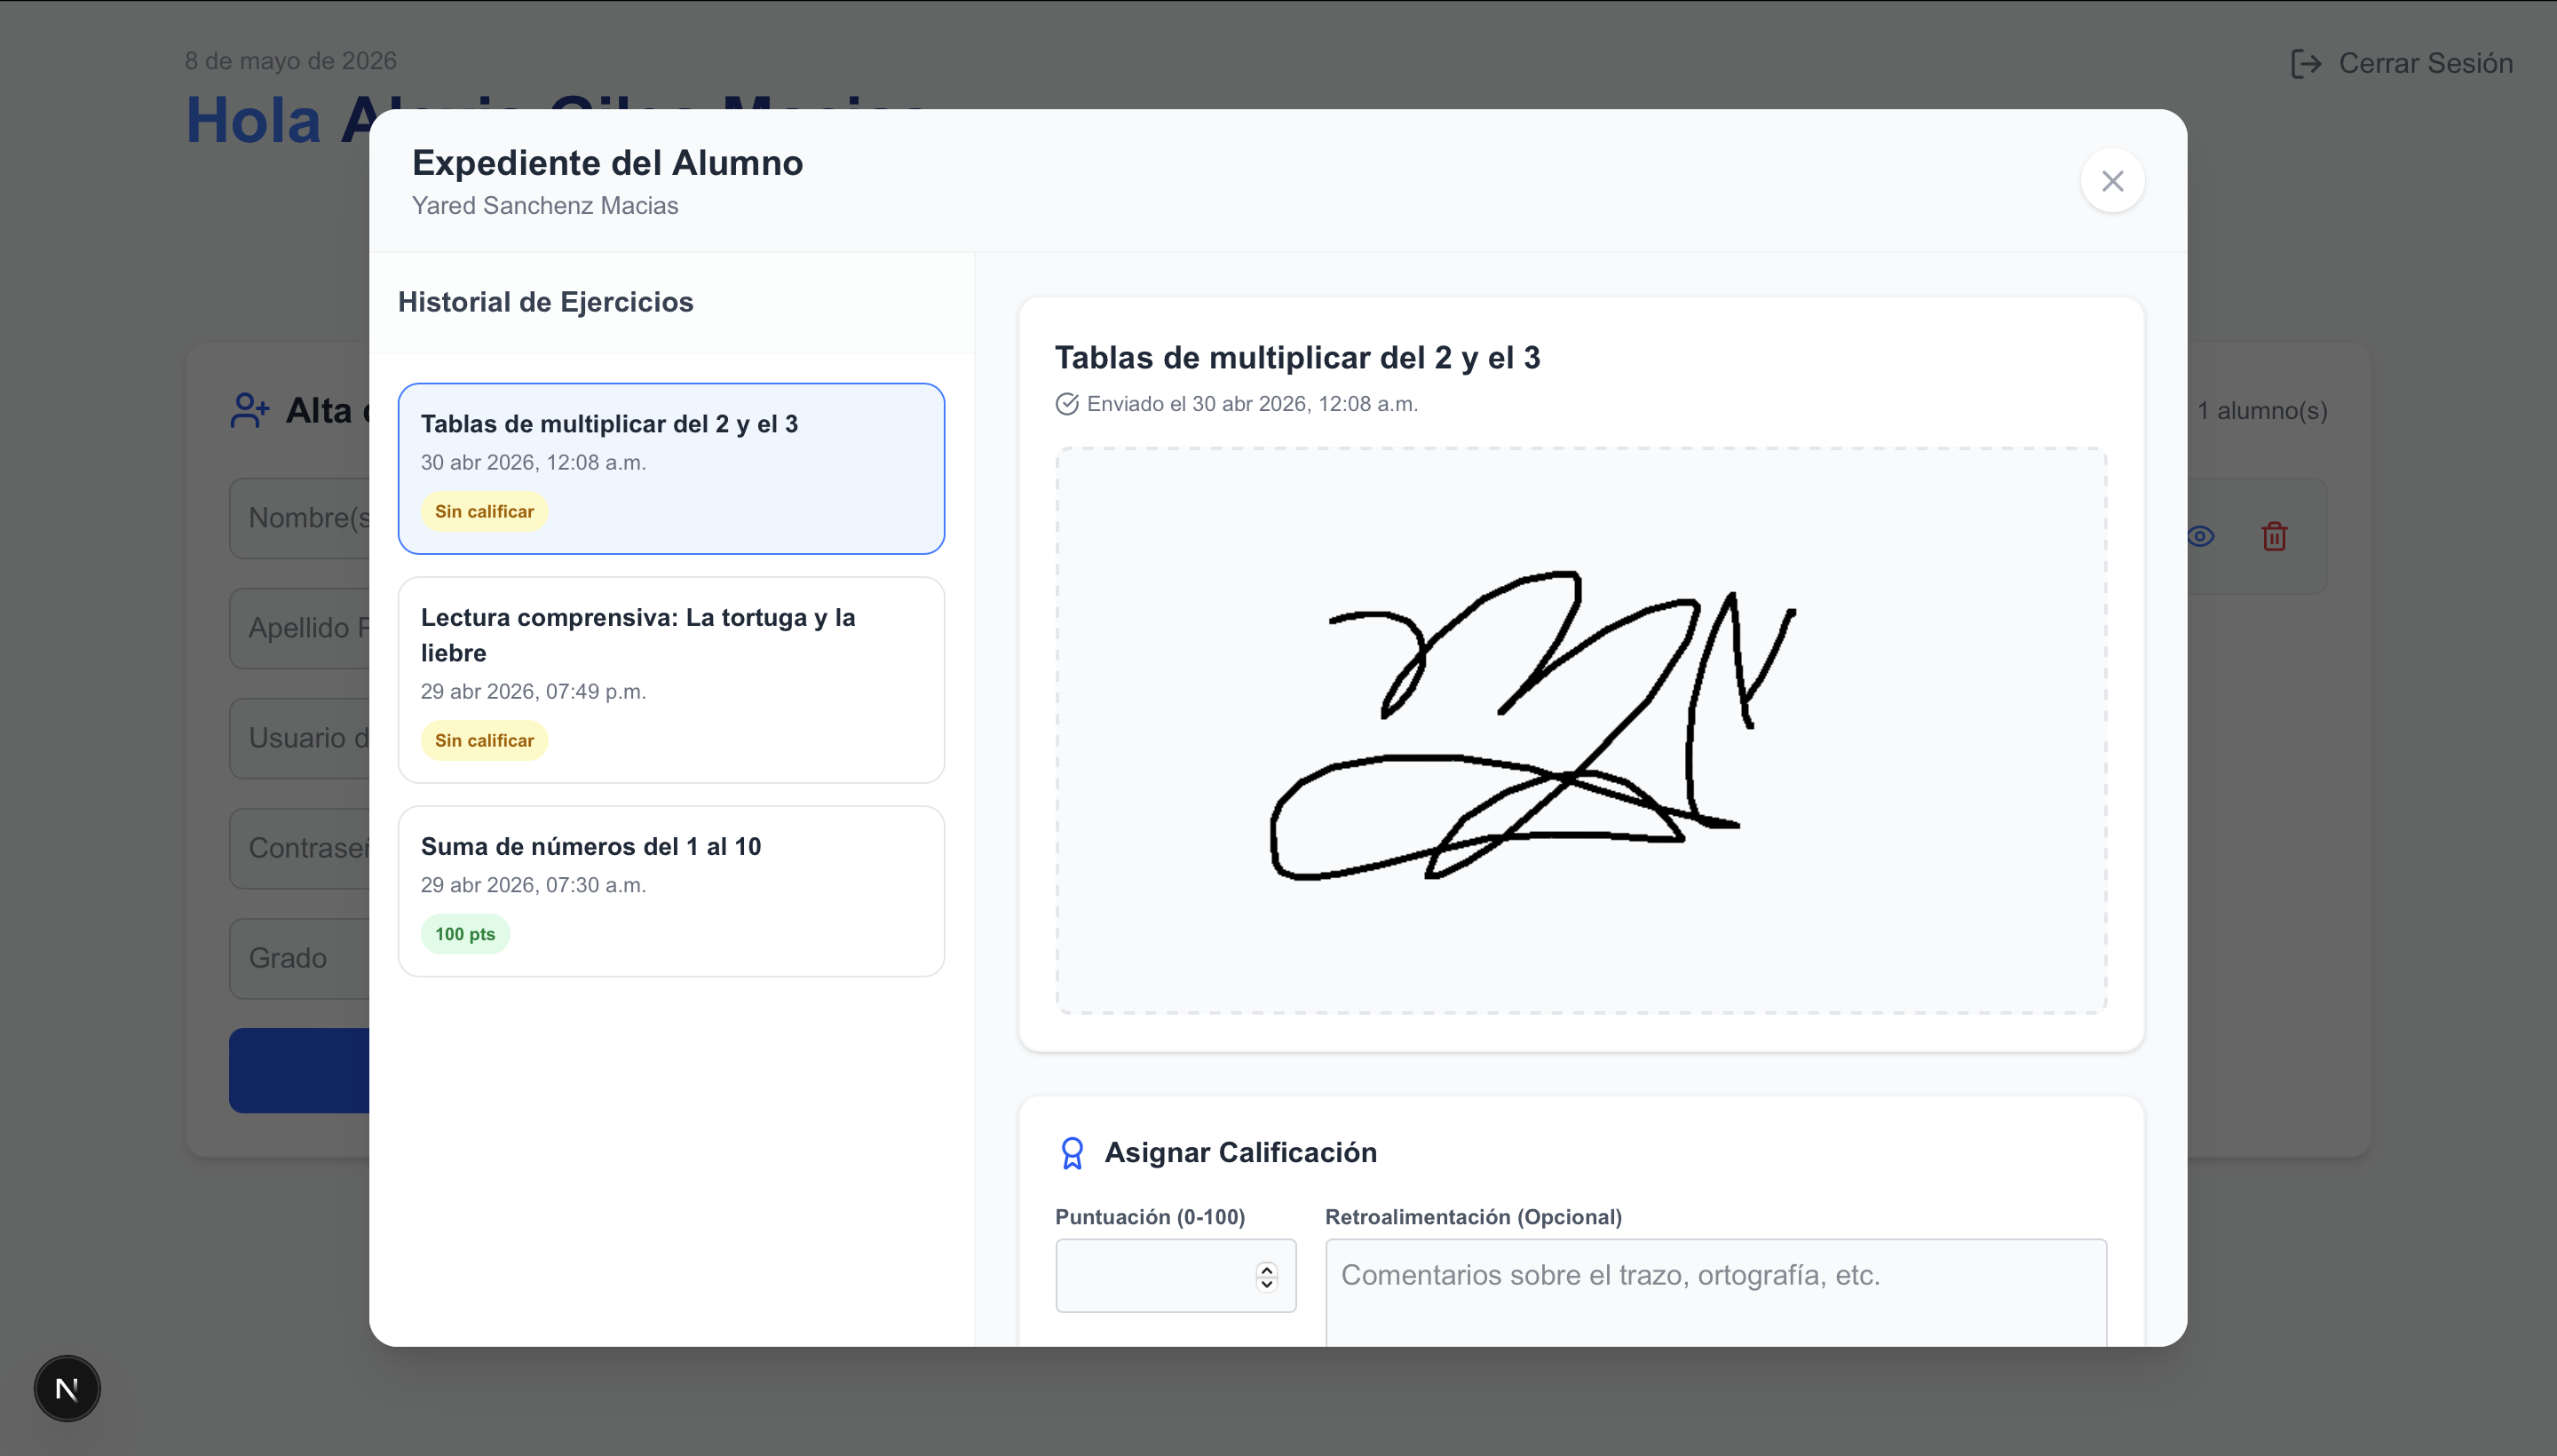
\includegraphics[width=0.7\textwidth]{Imagenes/historialAlumnos.png}
    \caption{Visualizacion del historial de ejercicios realizados por los alumnos}
    \label{fig:historialAlumnos}
\end{figure}

\begin{figure}[H]
    \centering
    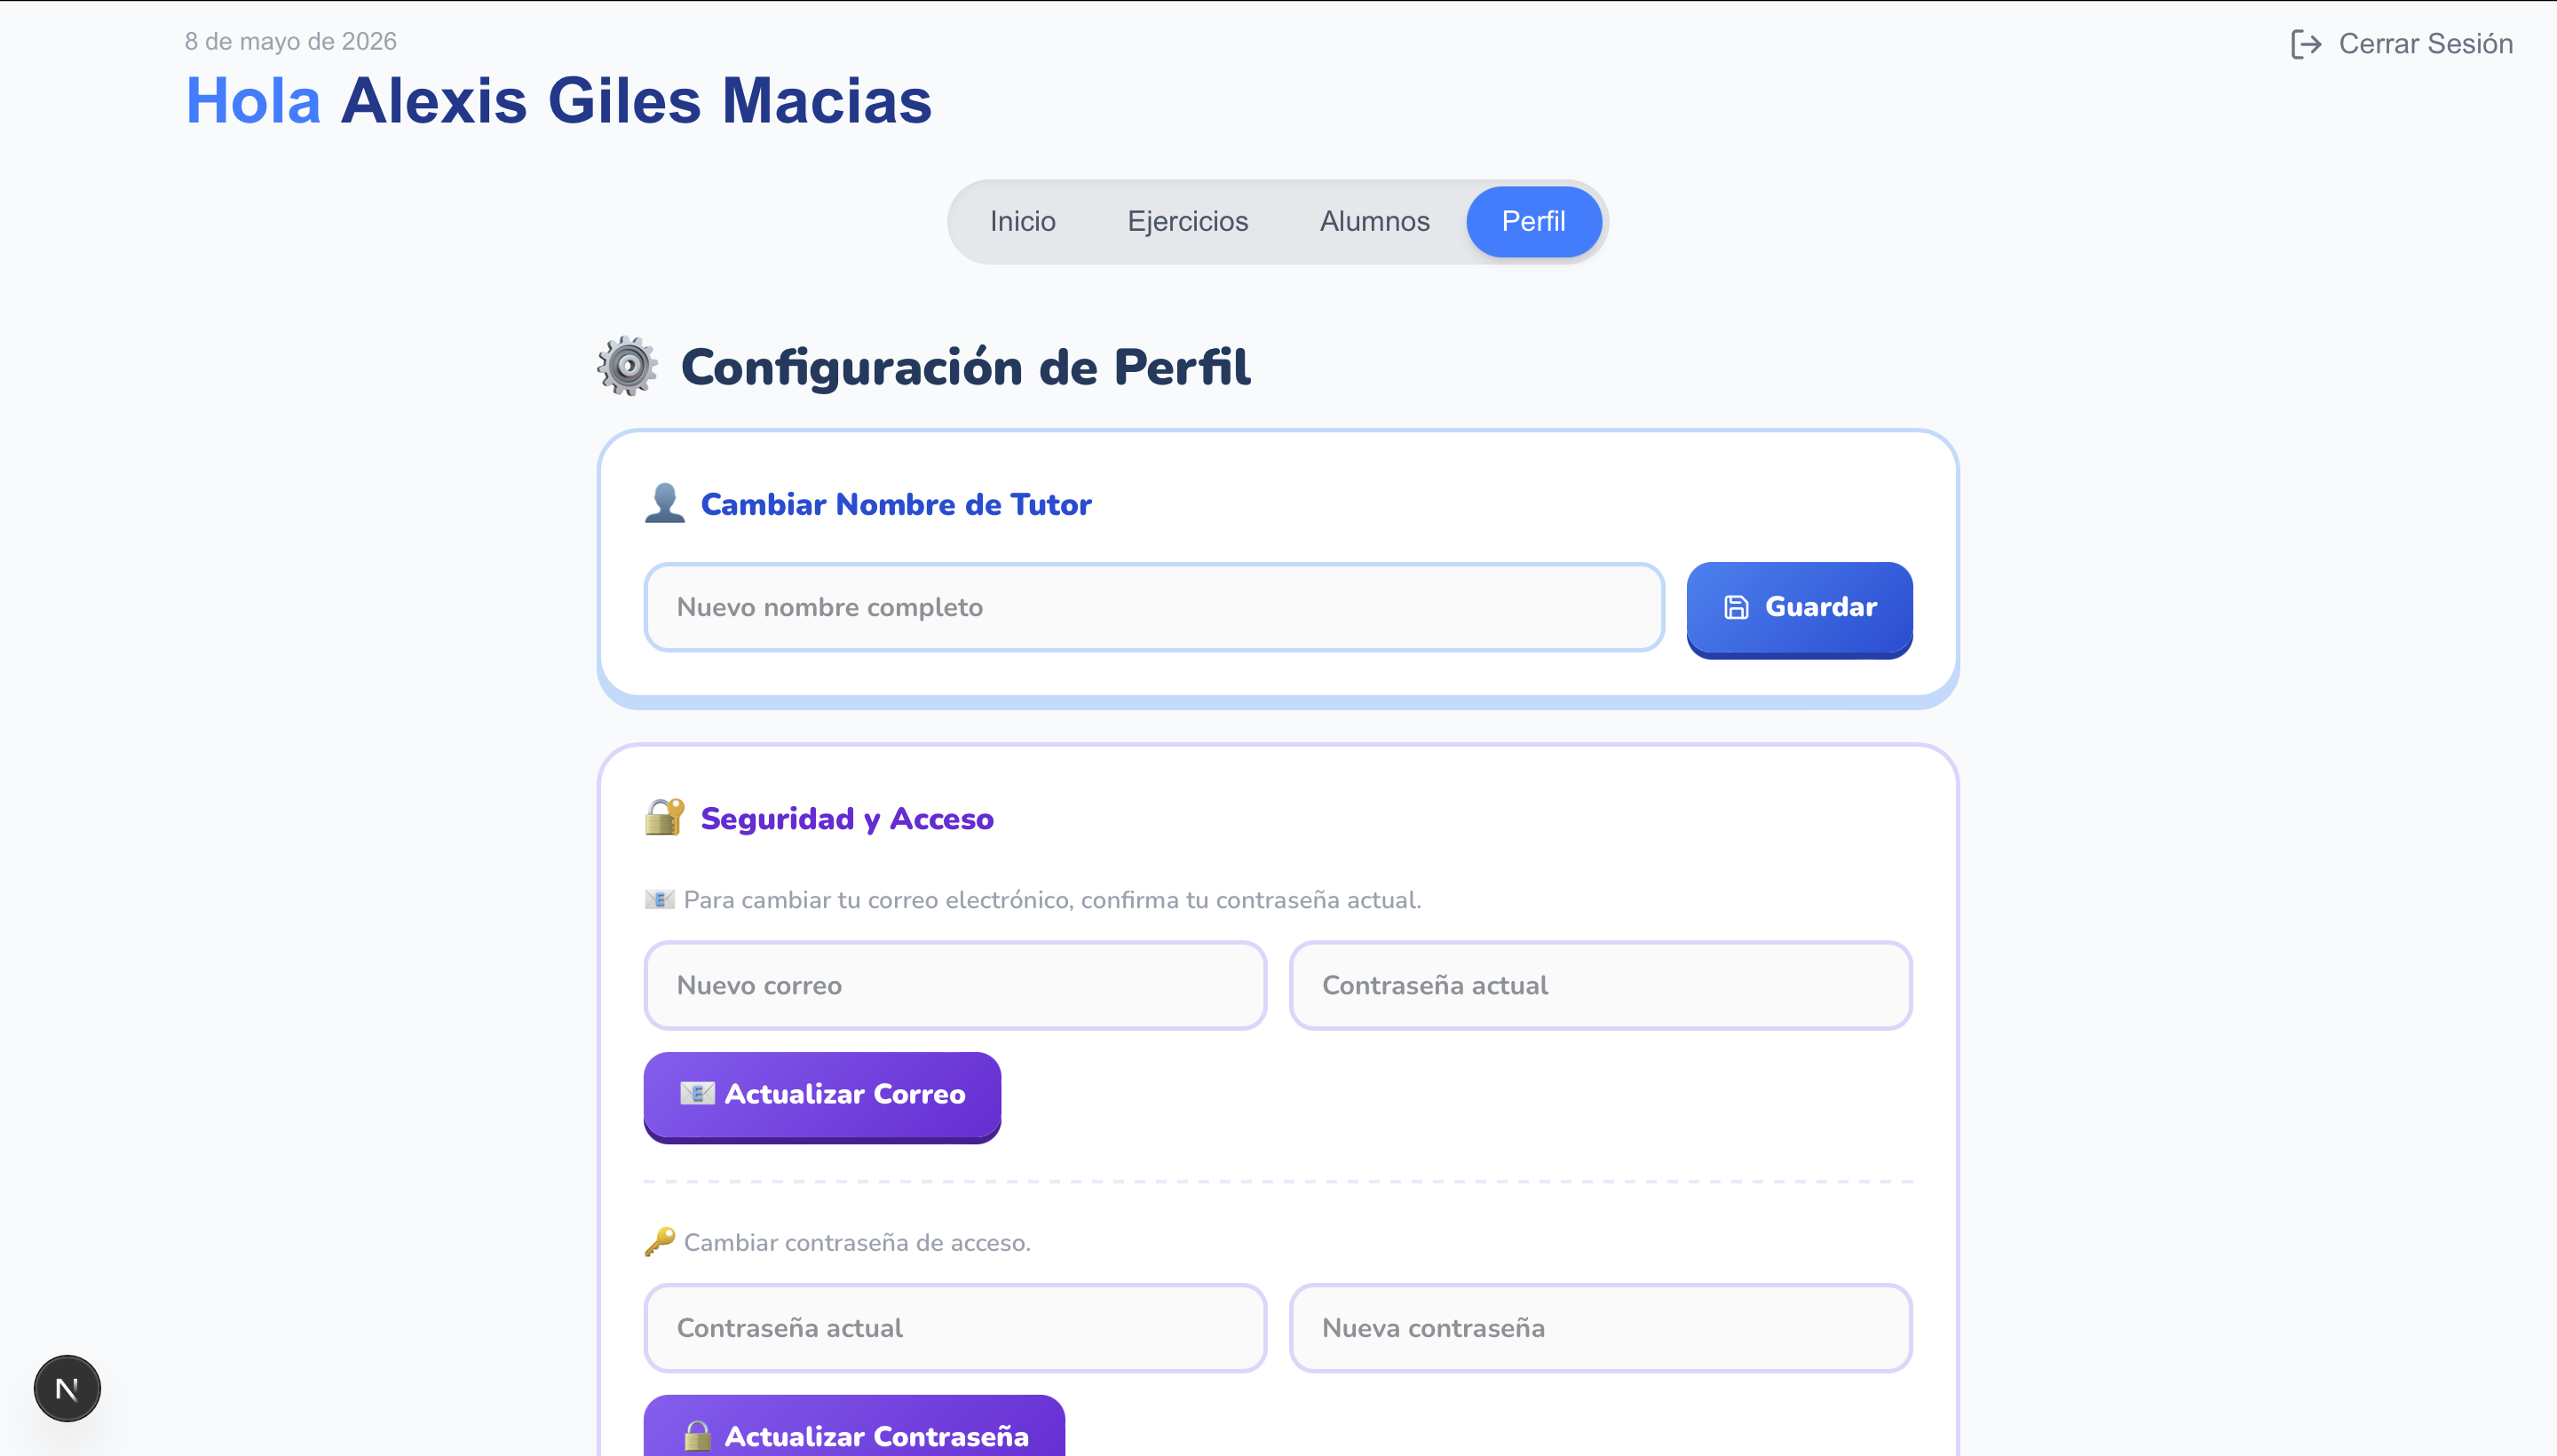
\includegraphics[width=0.7\textwidth]{Imagenes/miperfil.png}
    \caption{Visualizacion del perfil del tutor}
    \label{fig:miperfilT}
\end{figure}

\subsubsection{Vistas del alumno}

\begin{figure}[H]
    \centering
    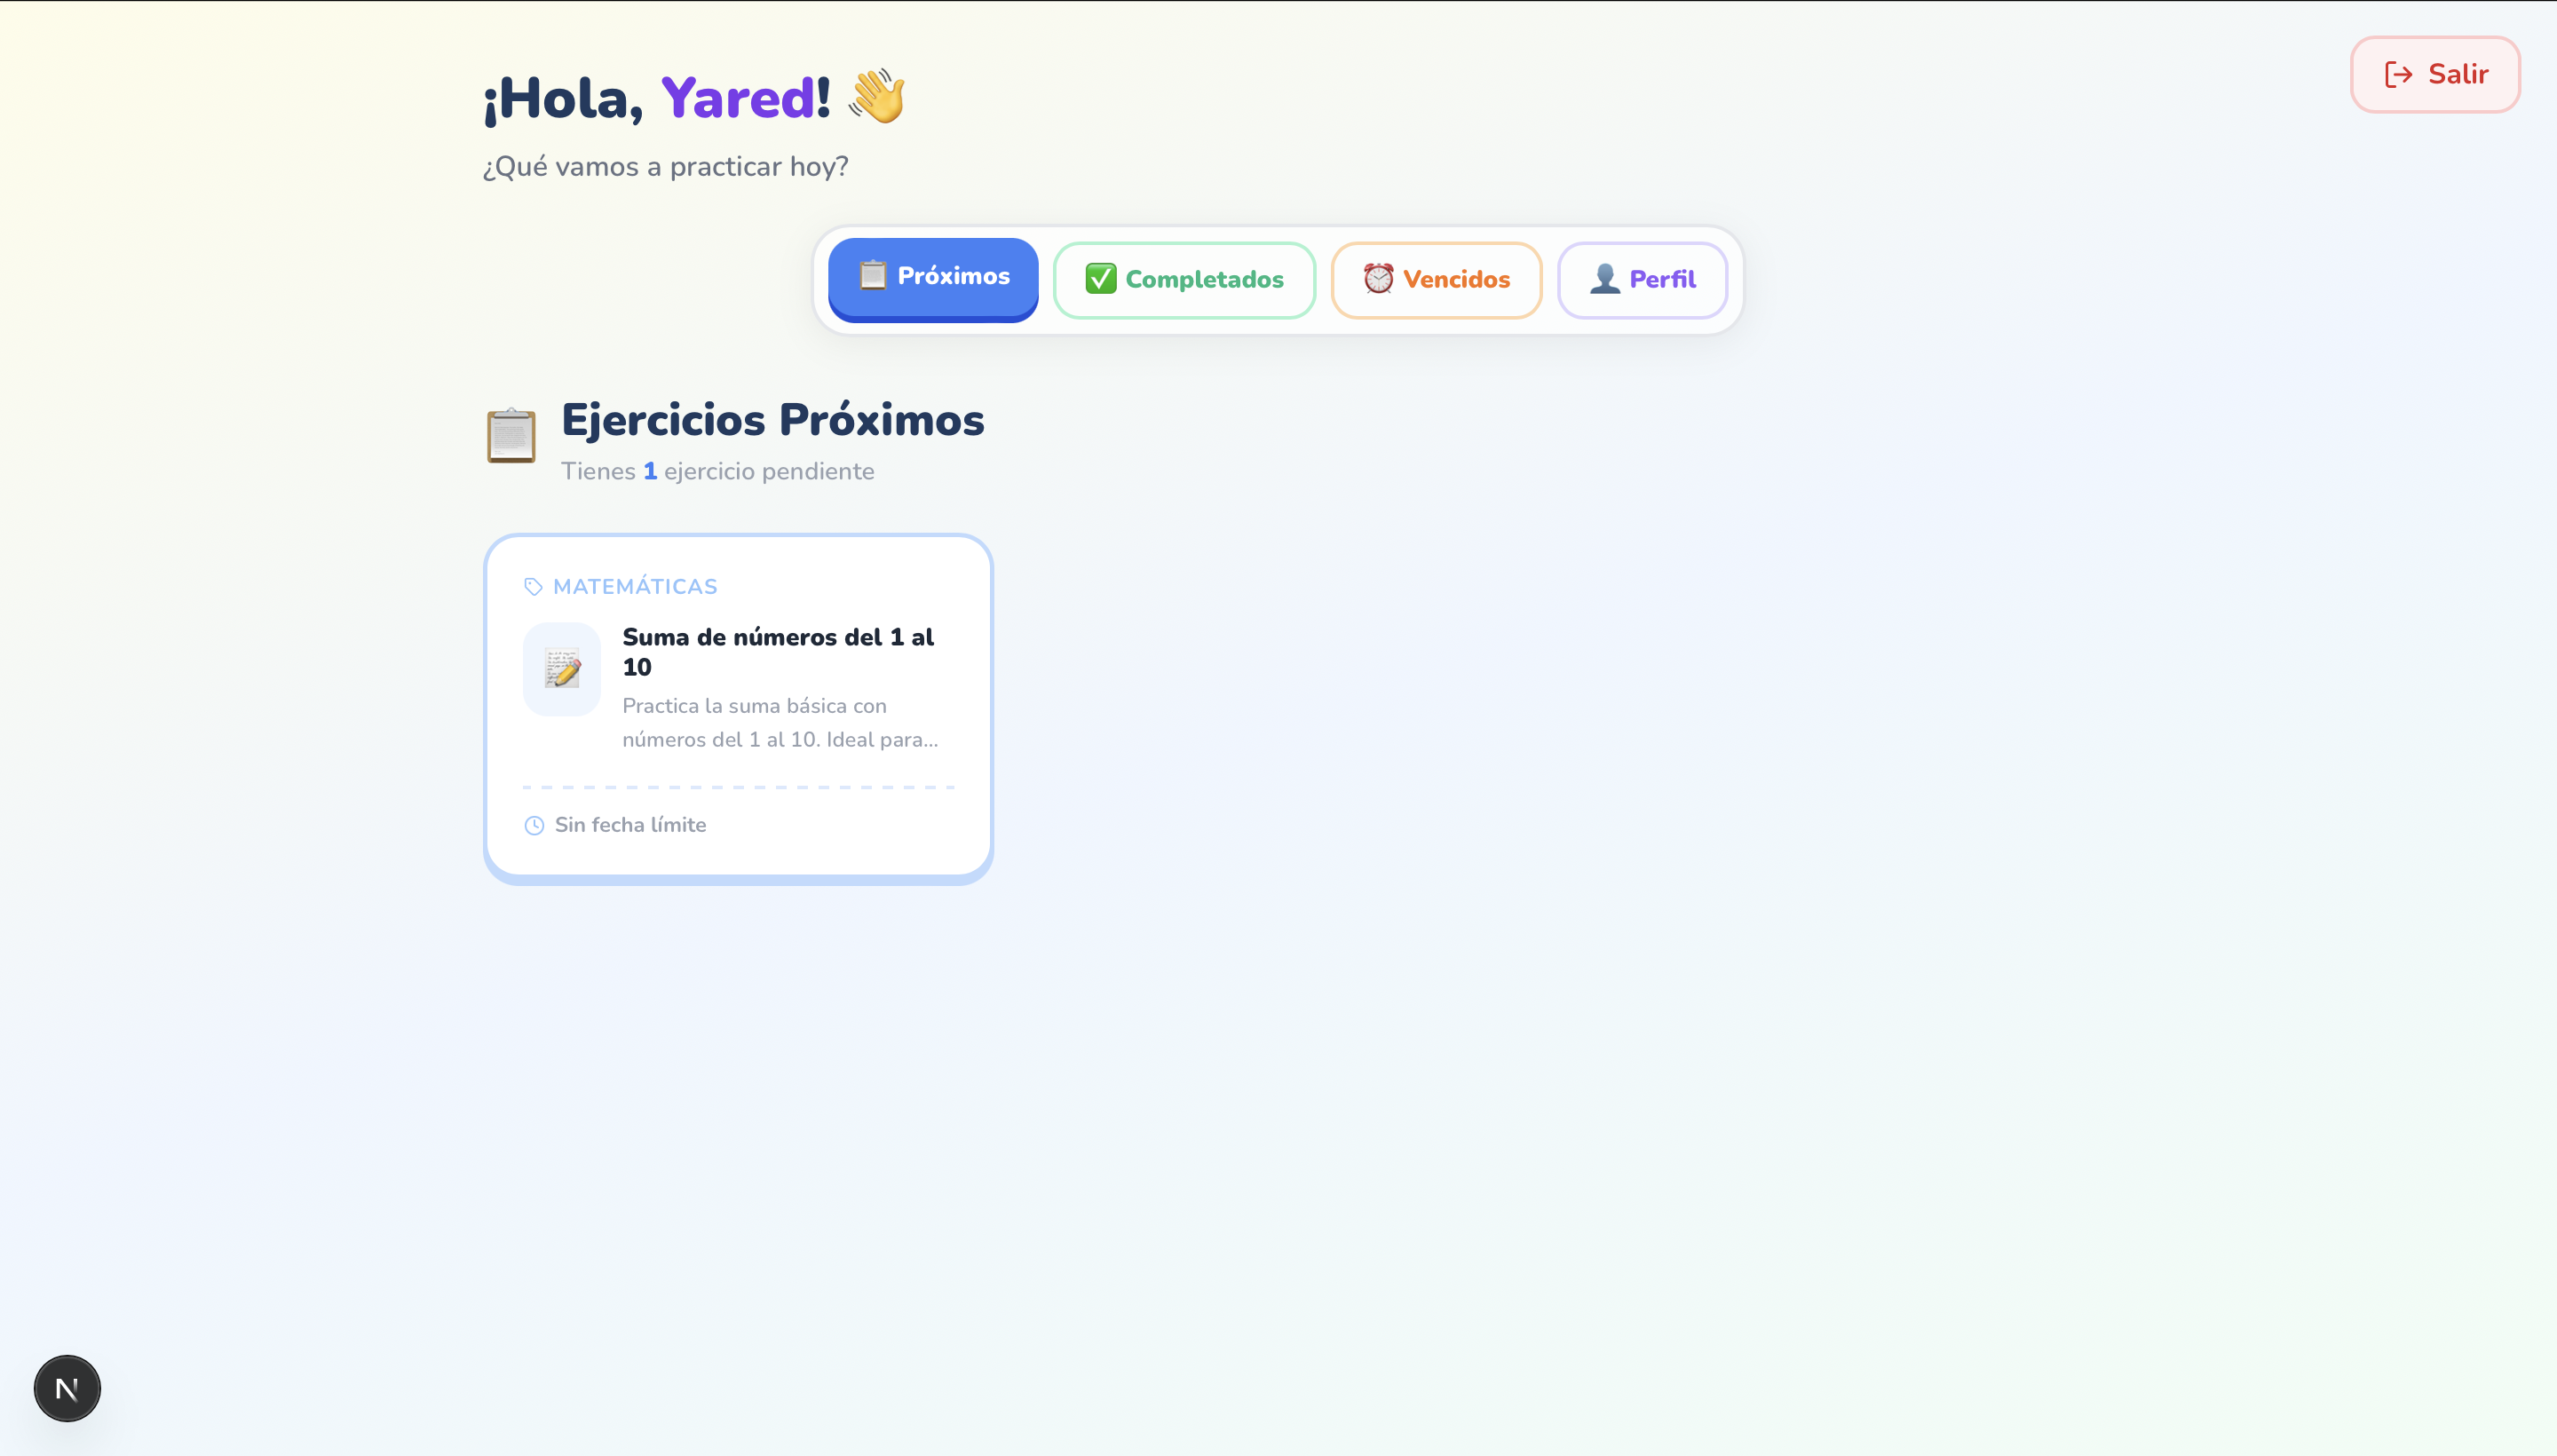
\includegraphics[width=0.7\textwidth]{Imagenes/ejerciciosProximos.png}
    \caption{Visualización de ejercicios próximos a vencer}
    \label{fig:ejerciciosProximos}
\end{figure}

\begin{figure}[H]
    \centering
    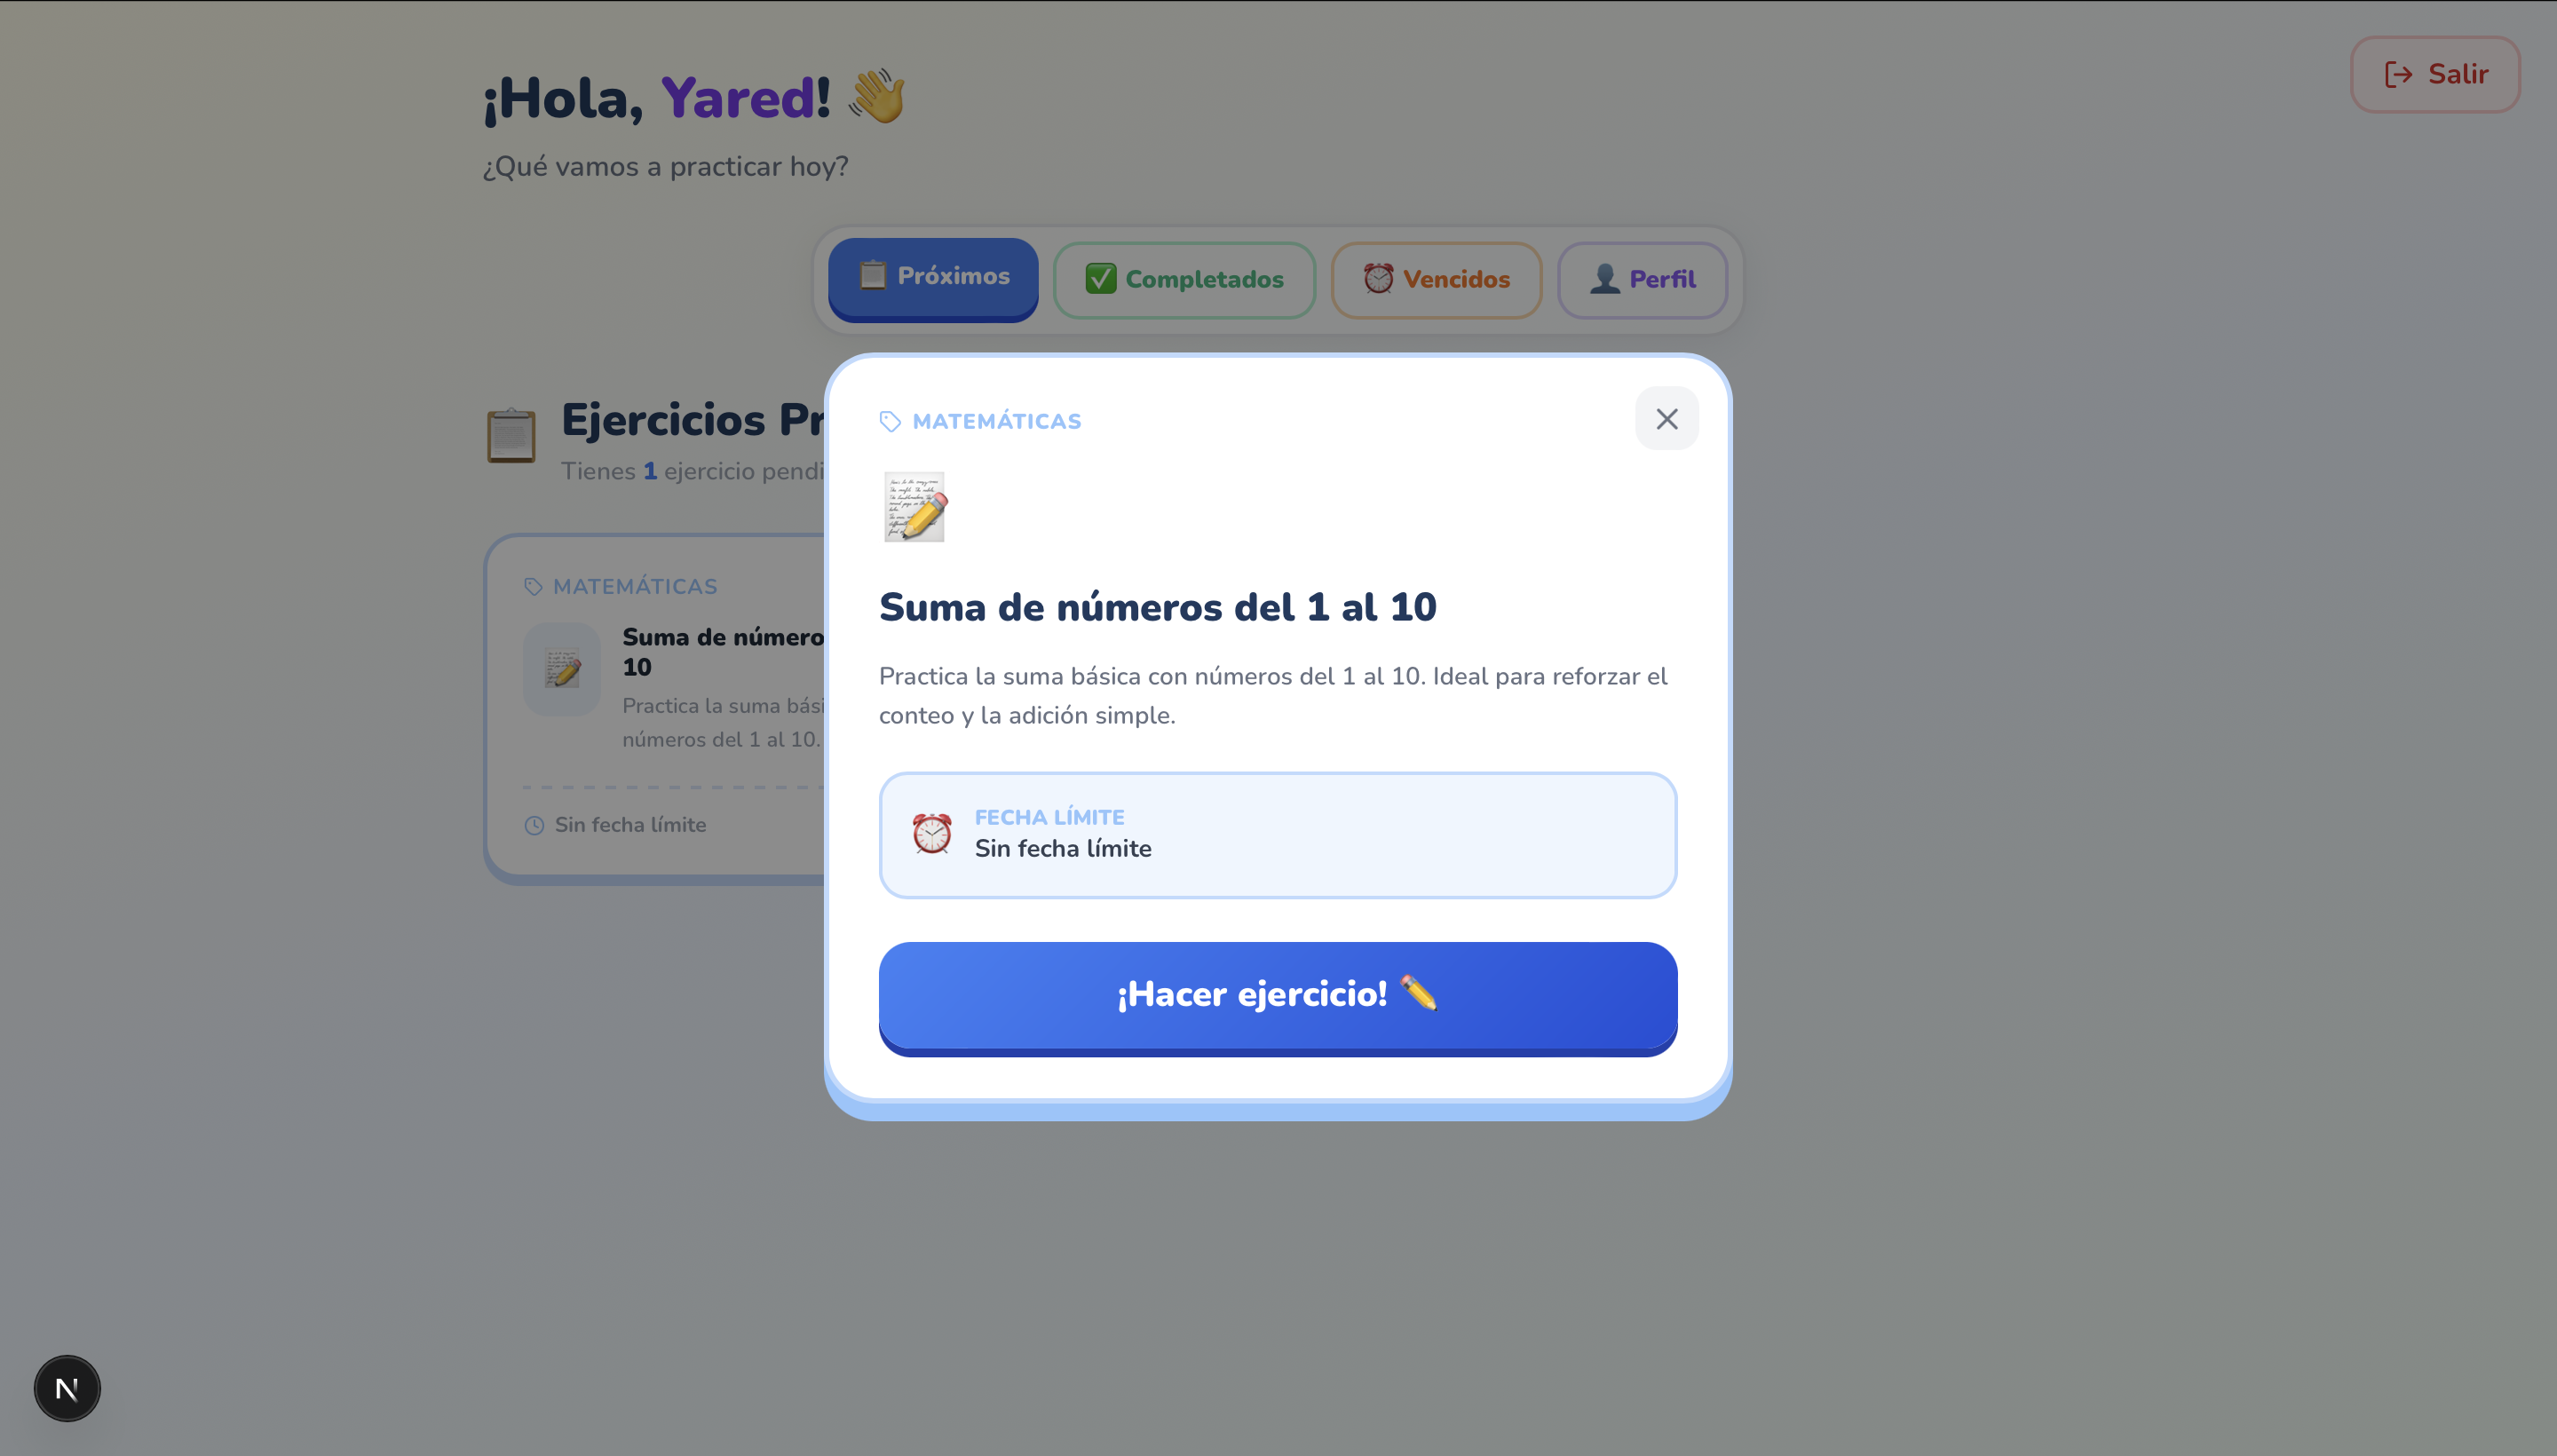
\includegraphics[width=0.7\textwidth]{Imagenes/seleccionEje.png}
    \caption{Visualización de ejercicio a realizar}
    \label{fig:seleccionEje}
\end{figure}

\begin{figure}[H]
    \centering
    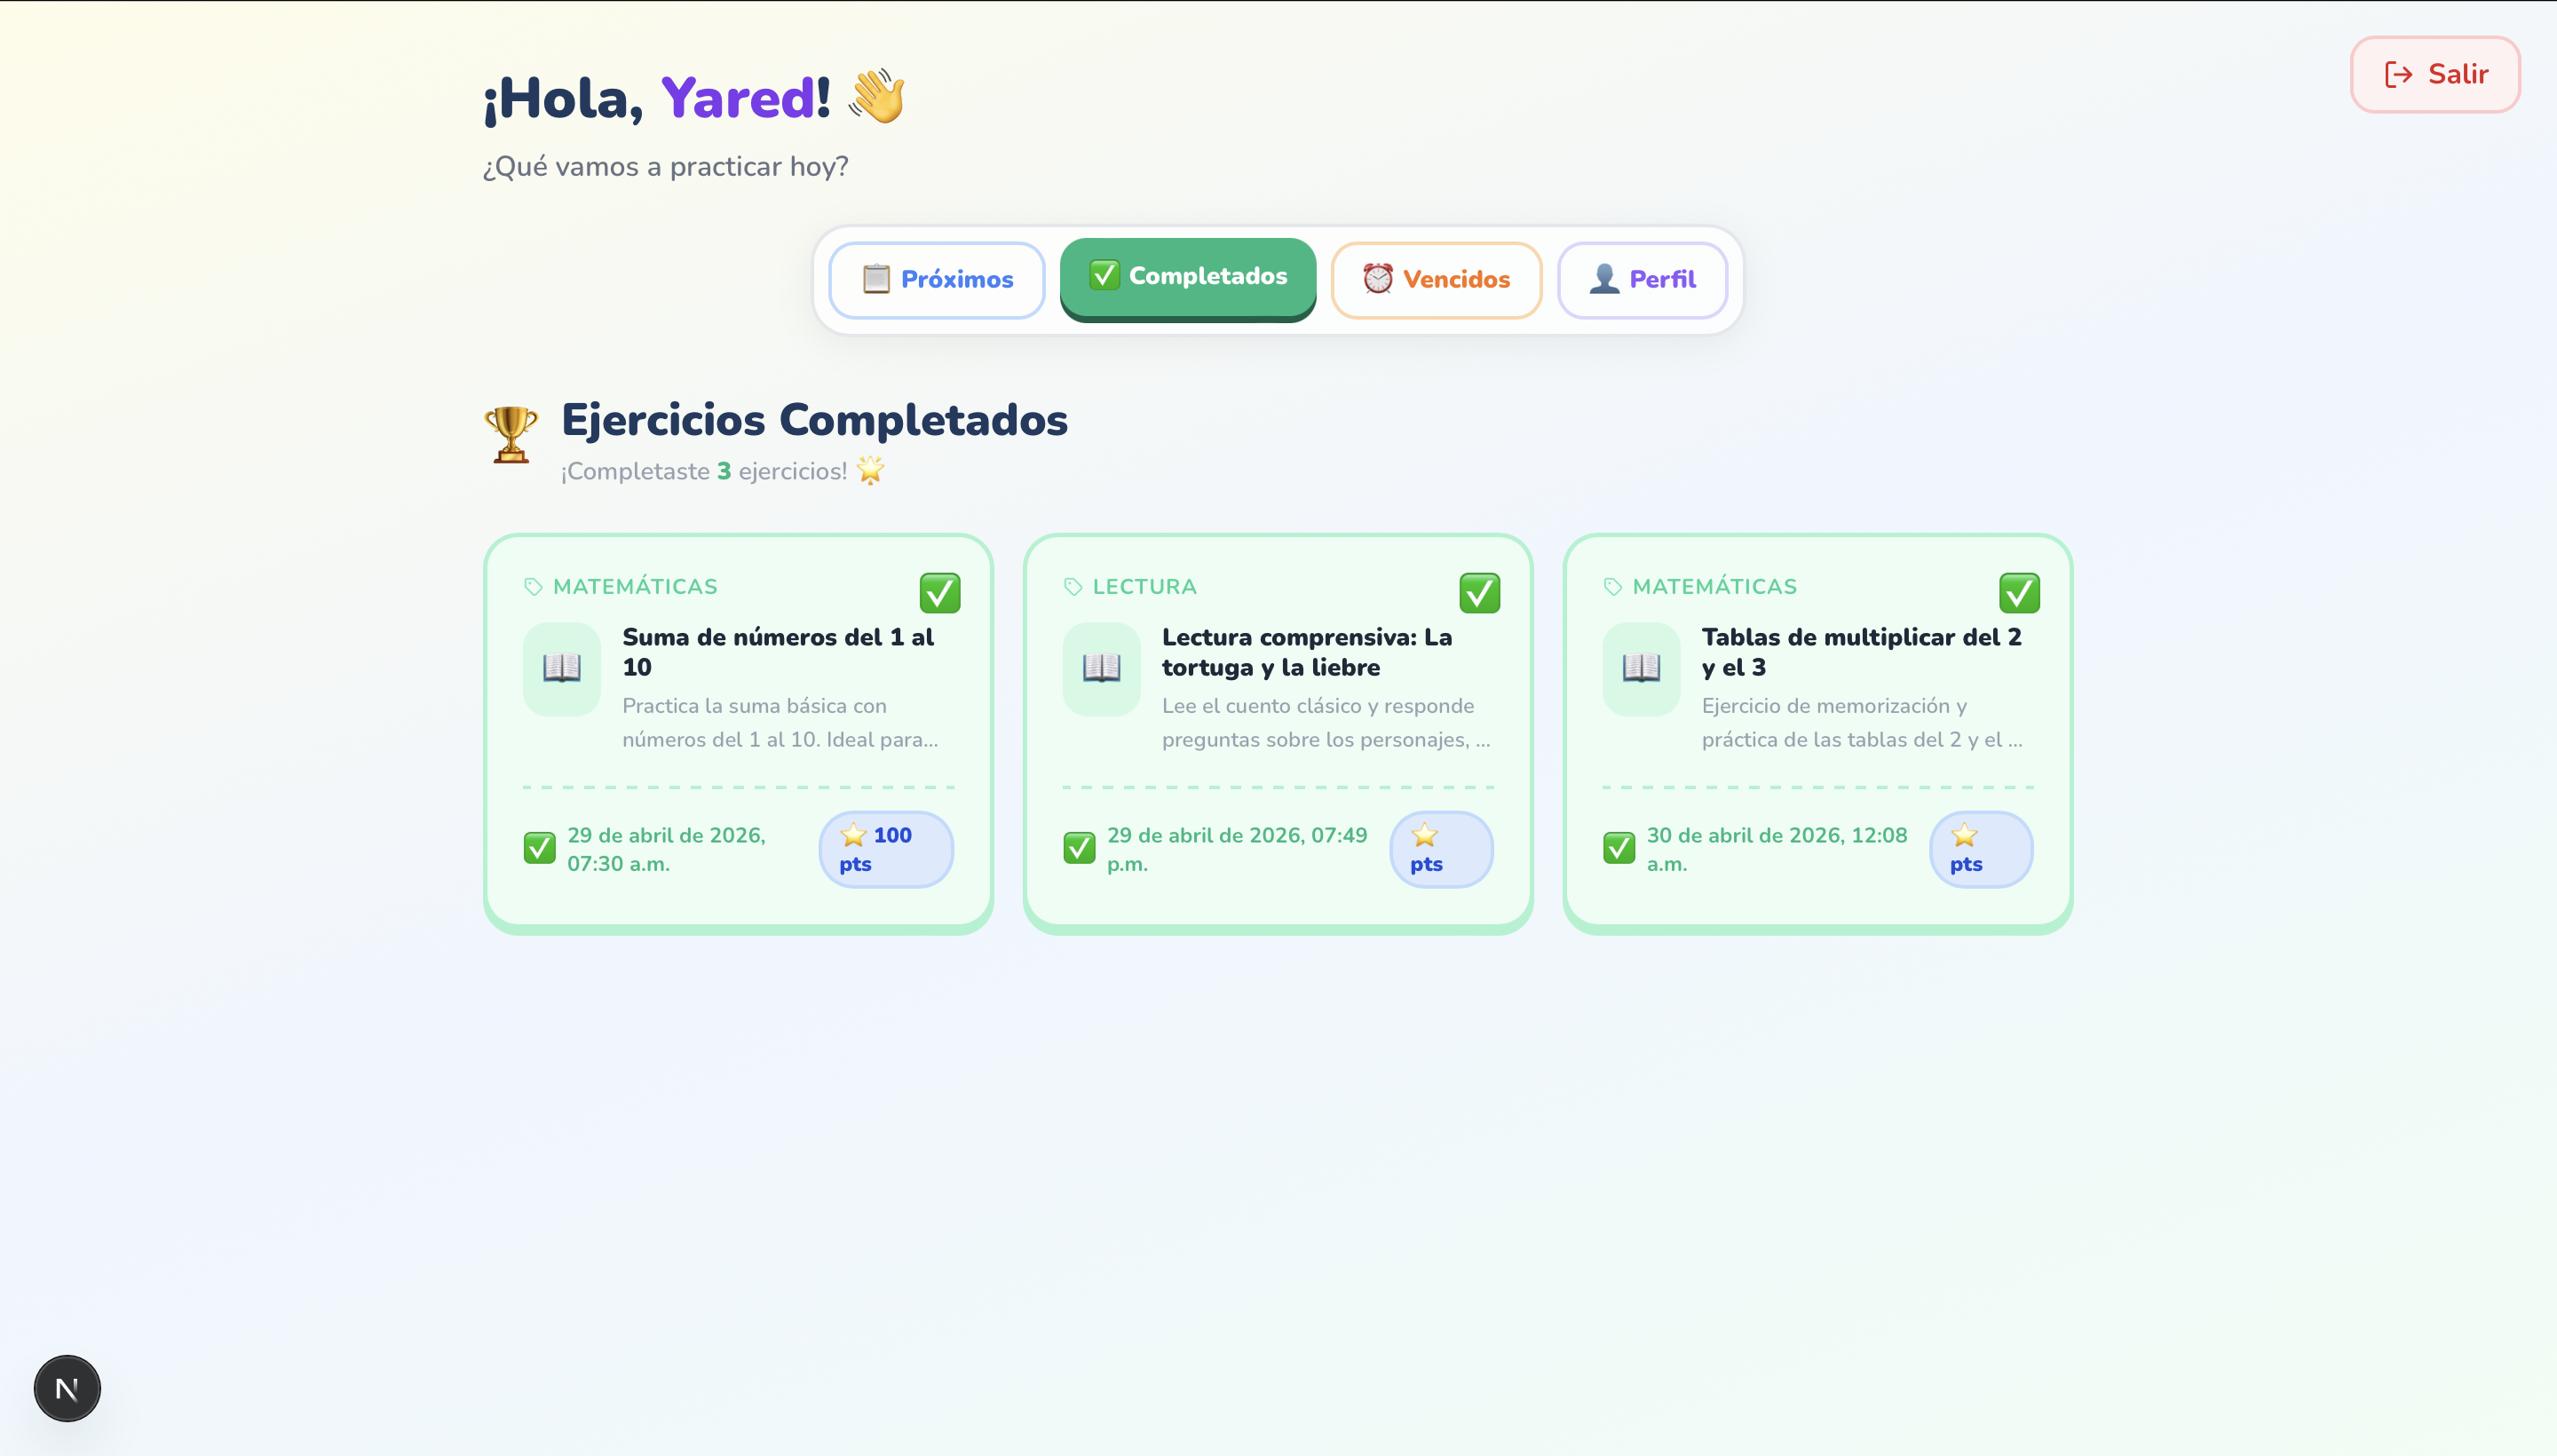
\includegraphics[width=0.7\textwidth]{Imagenes/ejerciciosCompletados.png}
    \caption{Visualización de ejercicios completados por el alumno}
    \label{fig:ejerciciosCompletados}
\end{figure}


\begin{figure}[H]
    \centering
    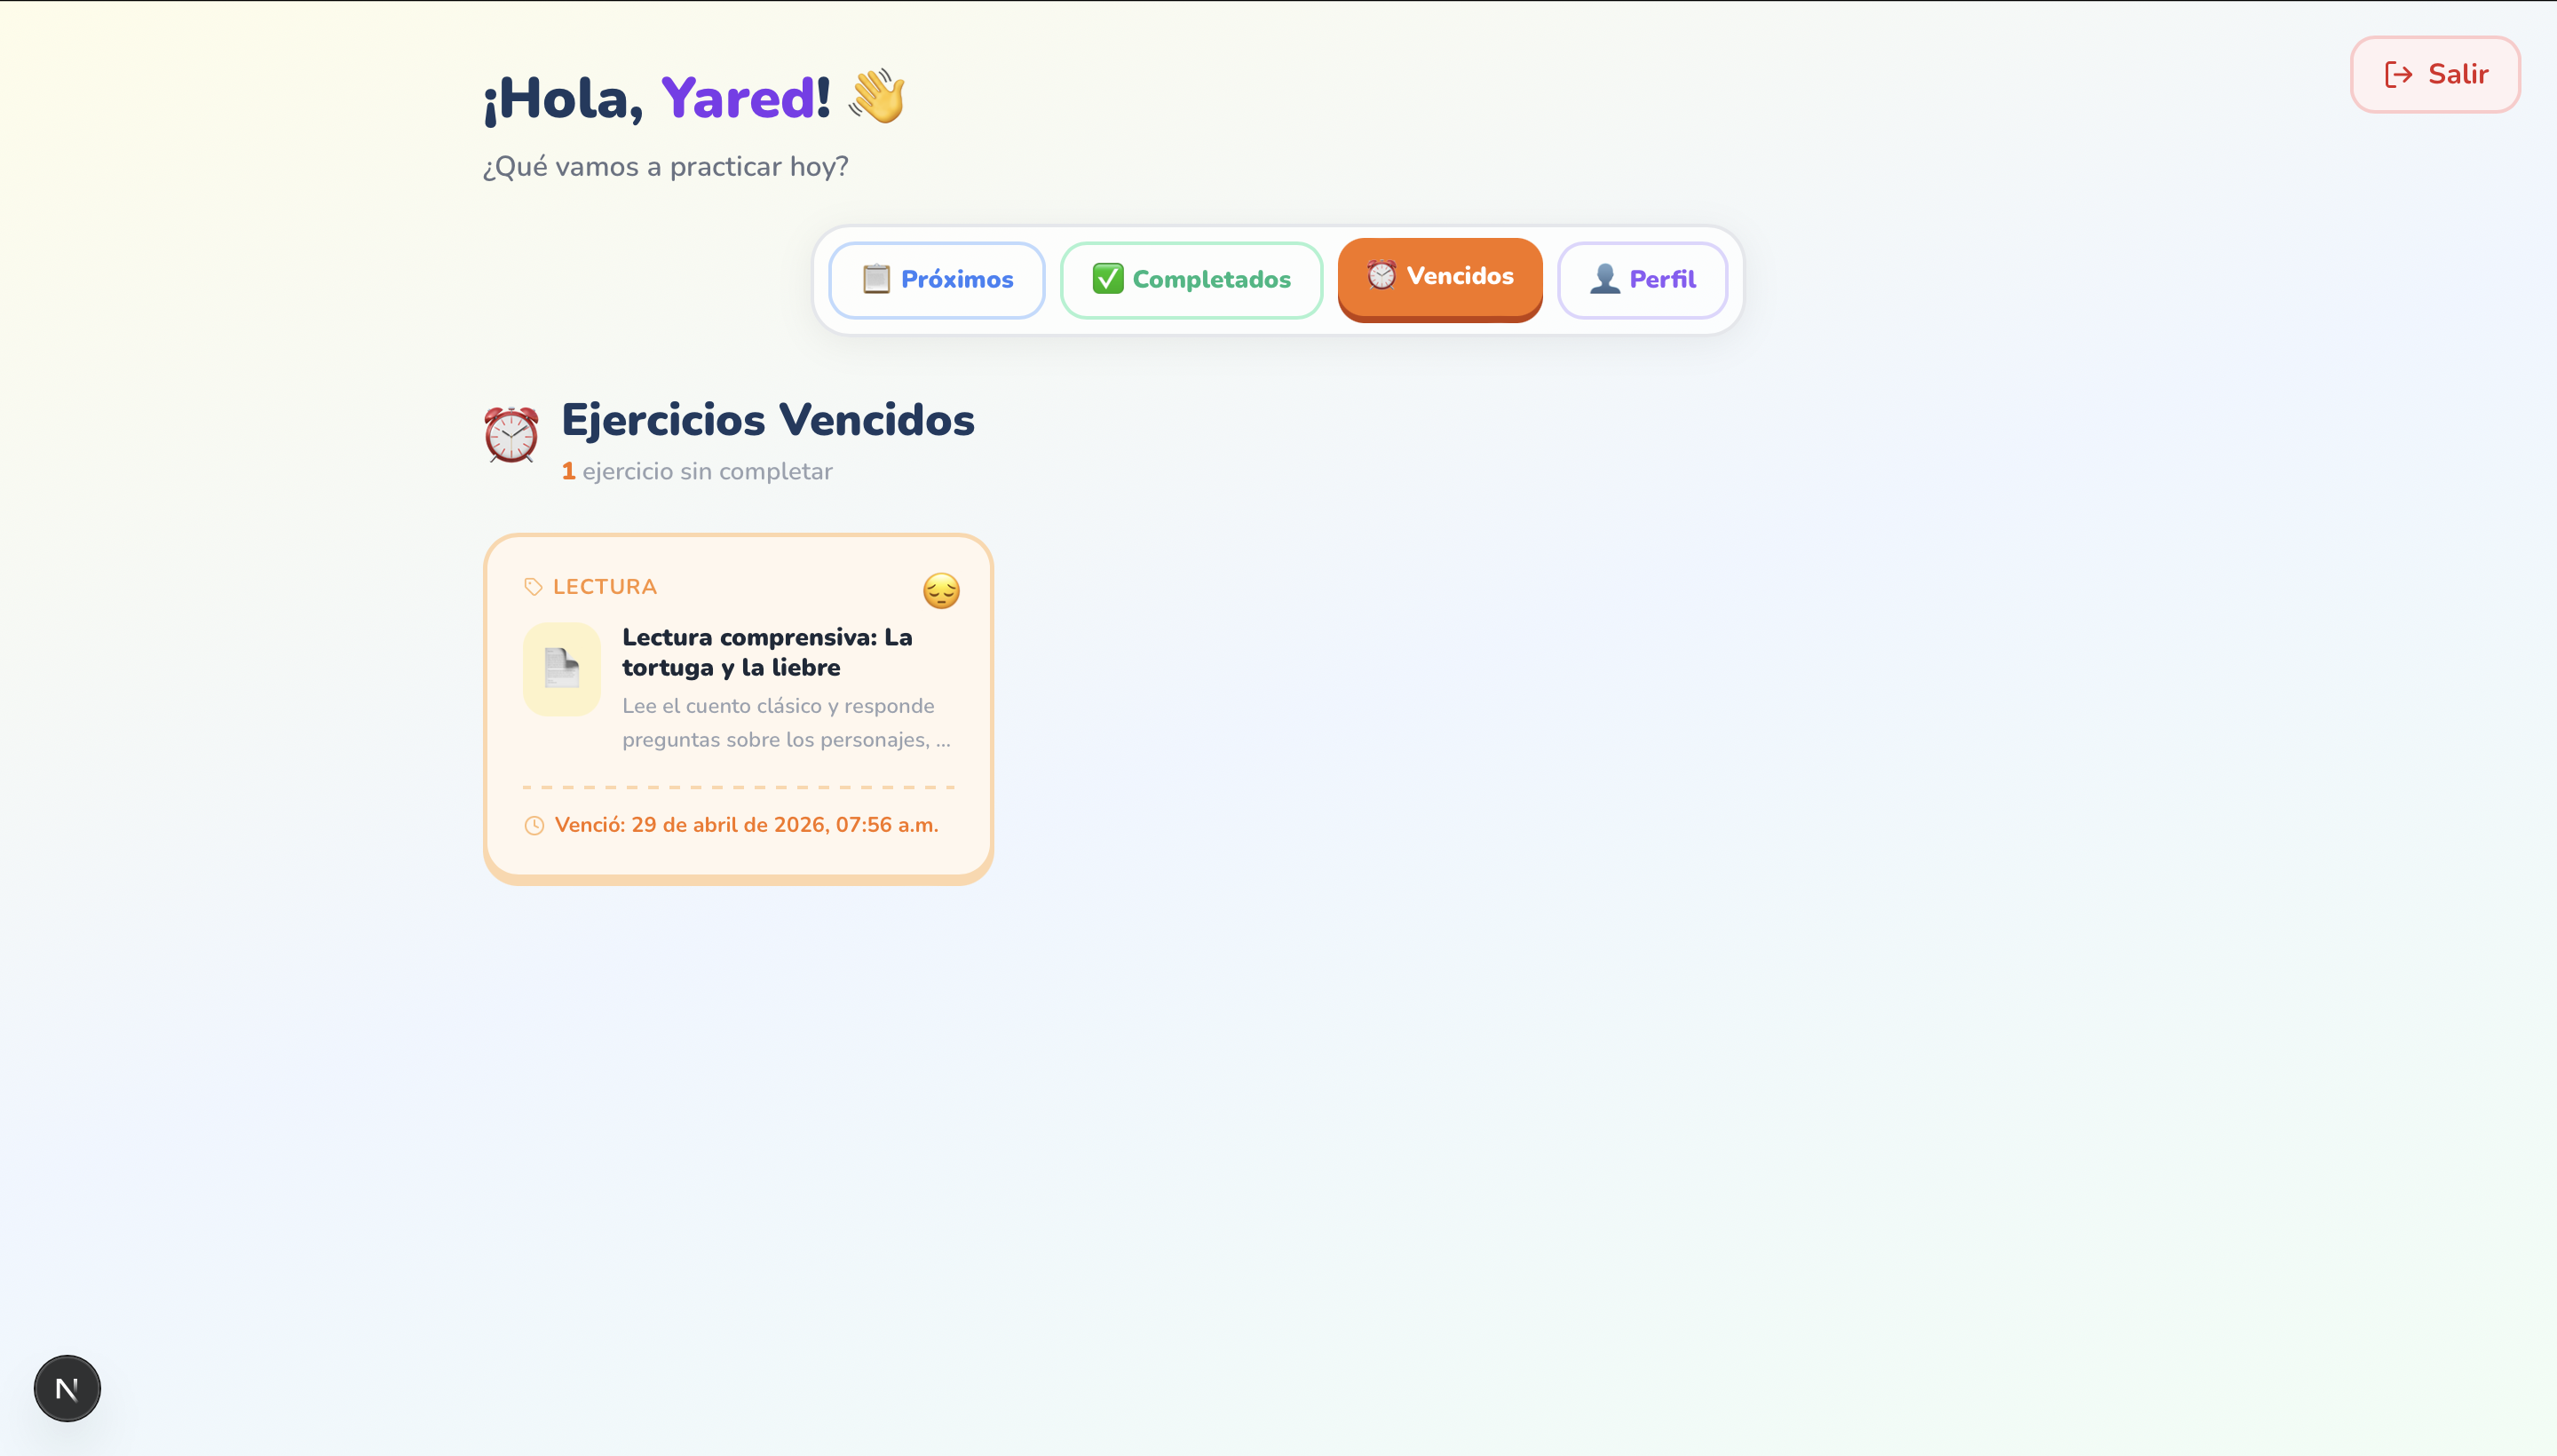
\includegraphics[width=0.7\textwidth]{Imagenes/ejerciciosVencidos.png}
    \caption{Visualización de ejercicios vencidos}
    \label{fig:ejerciciosVencidos}
\end{figure}

\begin{figure}[H]
    \centering
    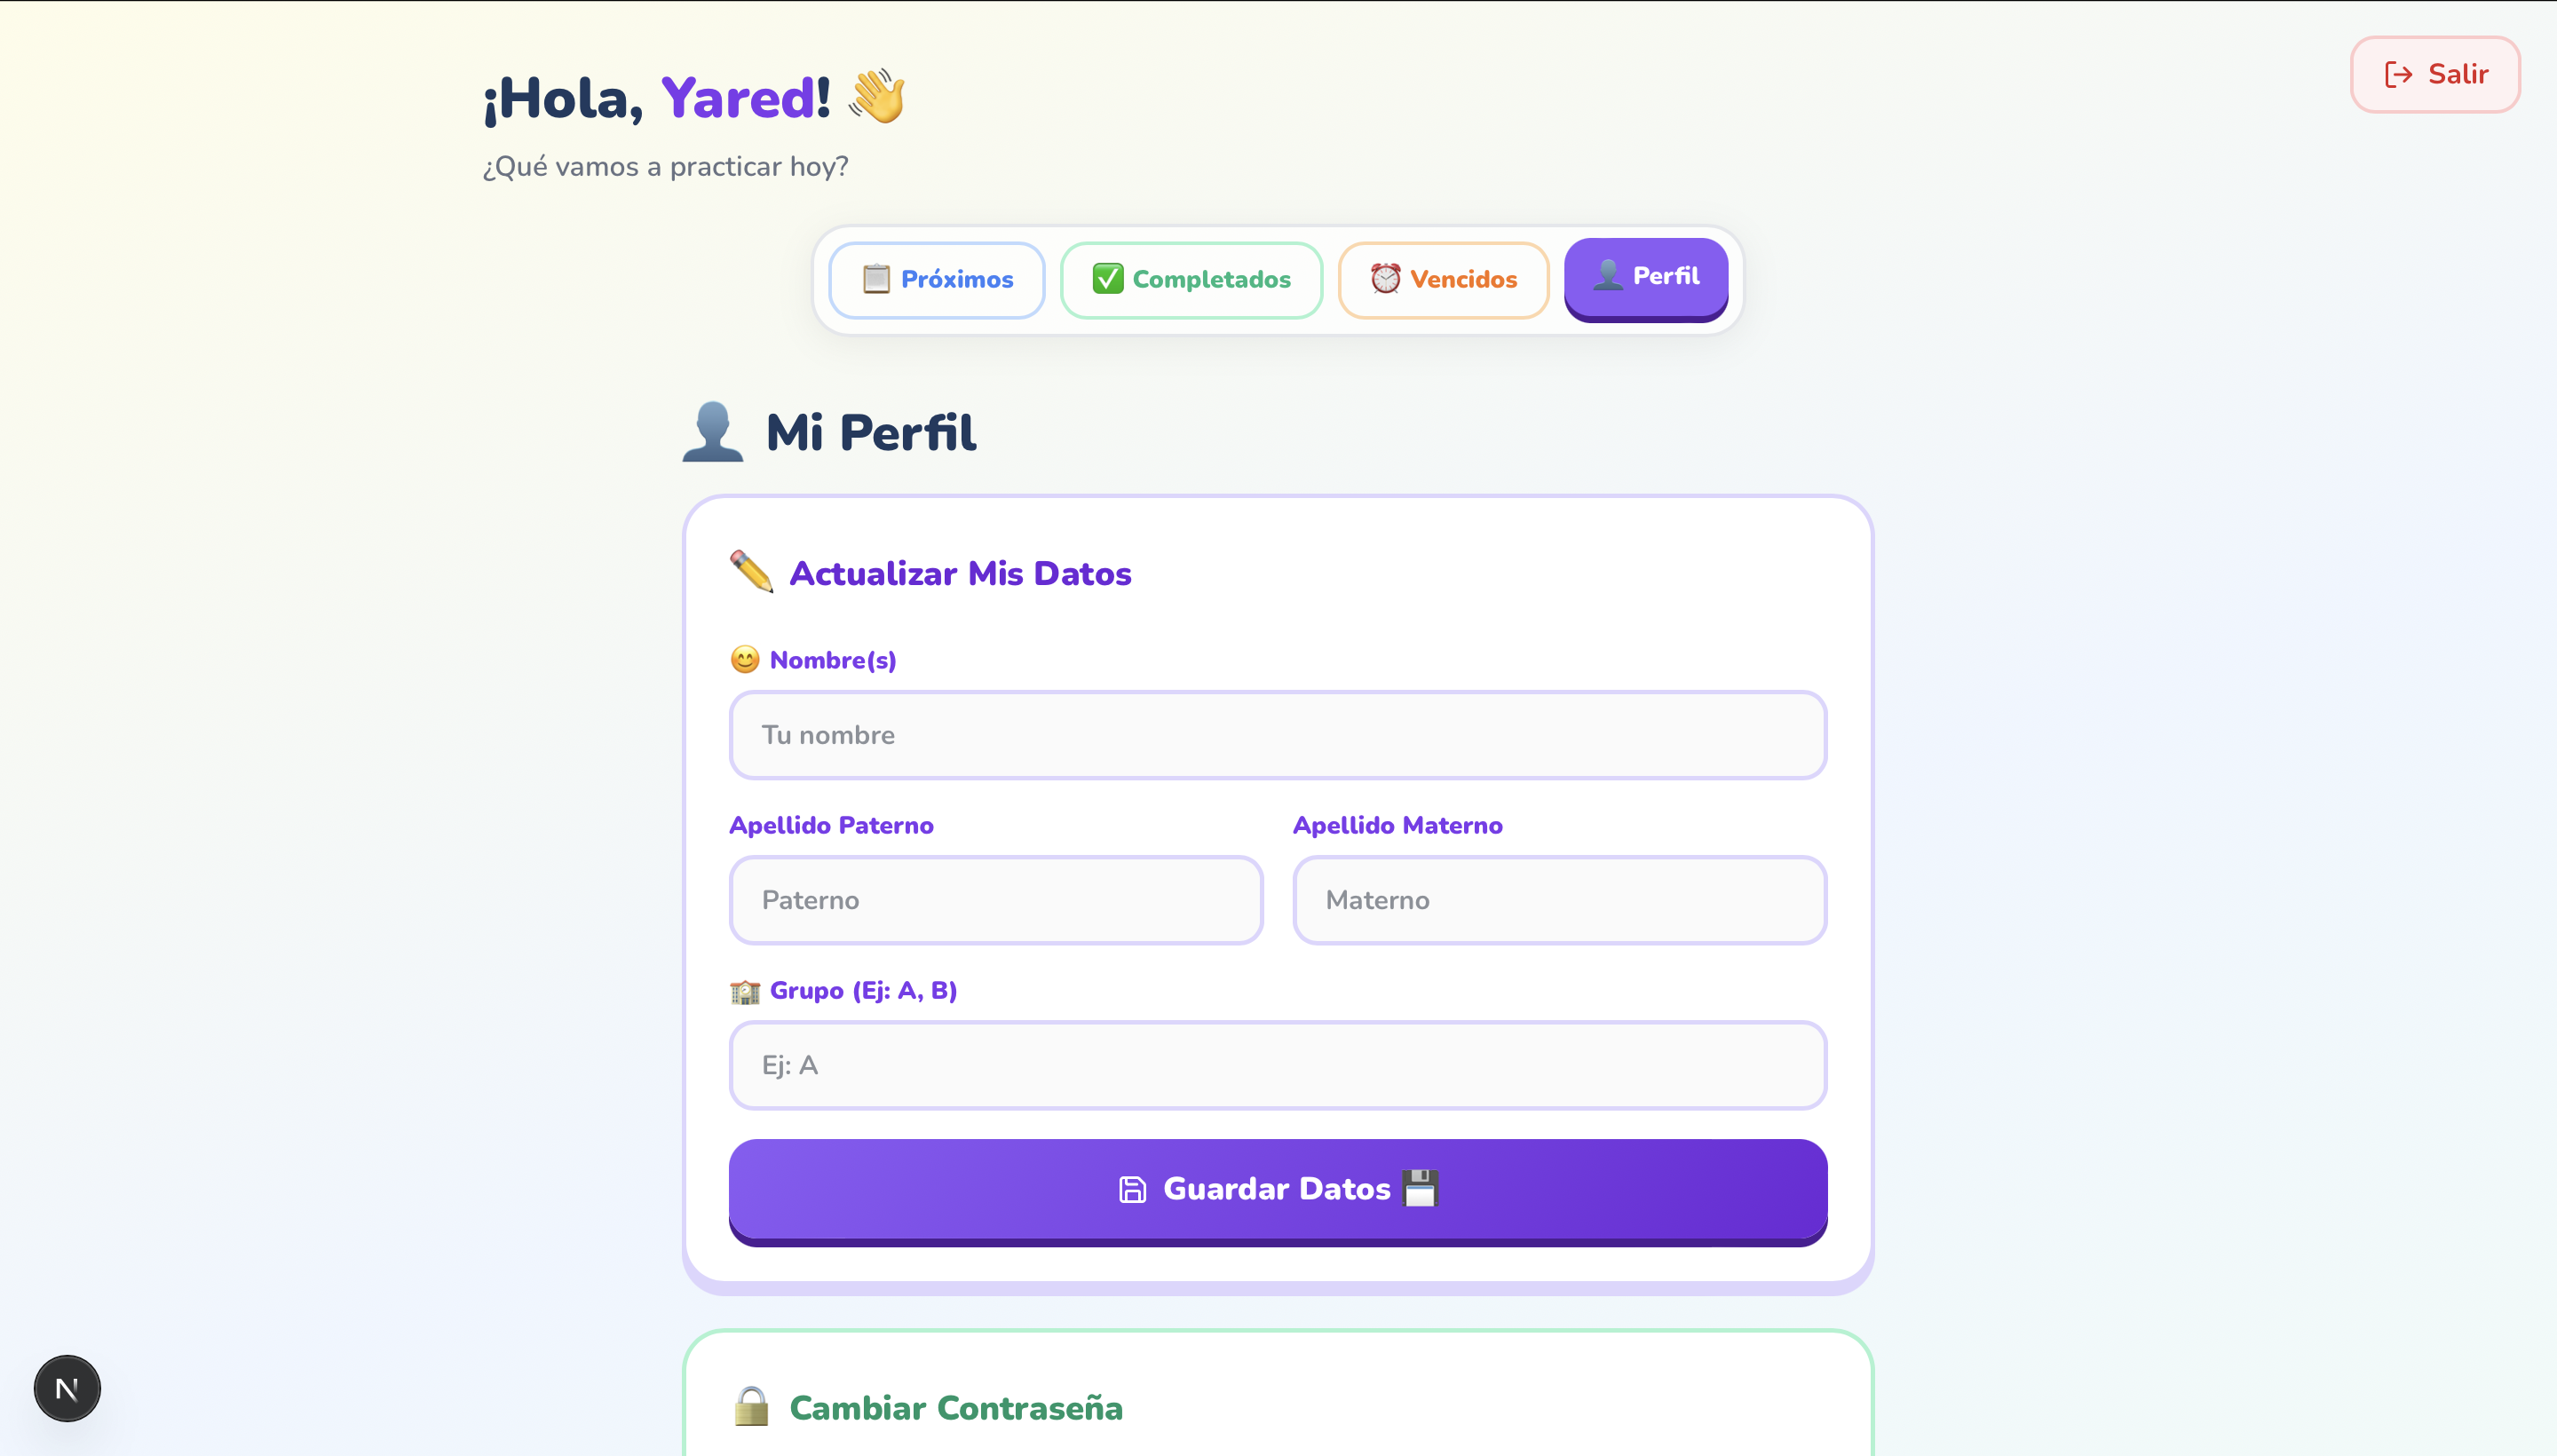
\includegraphics[width=0.7\textwidth]{Imagenes/miperfilA.png}
    \caption{Visualización del perfil del alumno}
    \label{fig:miperfilA}
\end{figure}

\subsubsection{Vista del lienzo digital}

\begin{figure}[H]
    \centering
    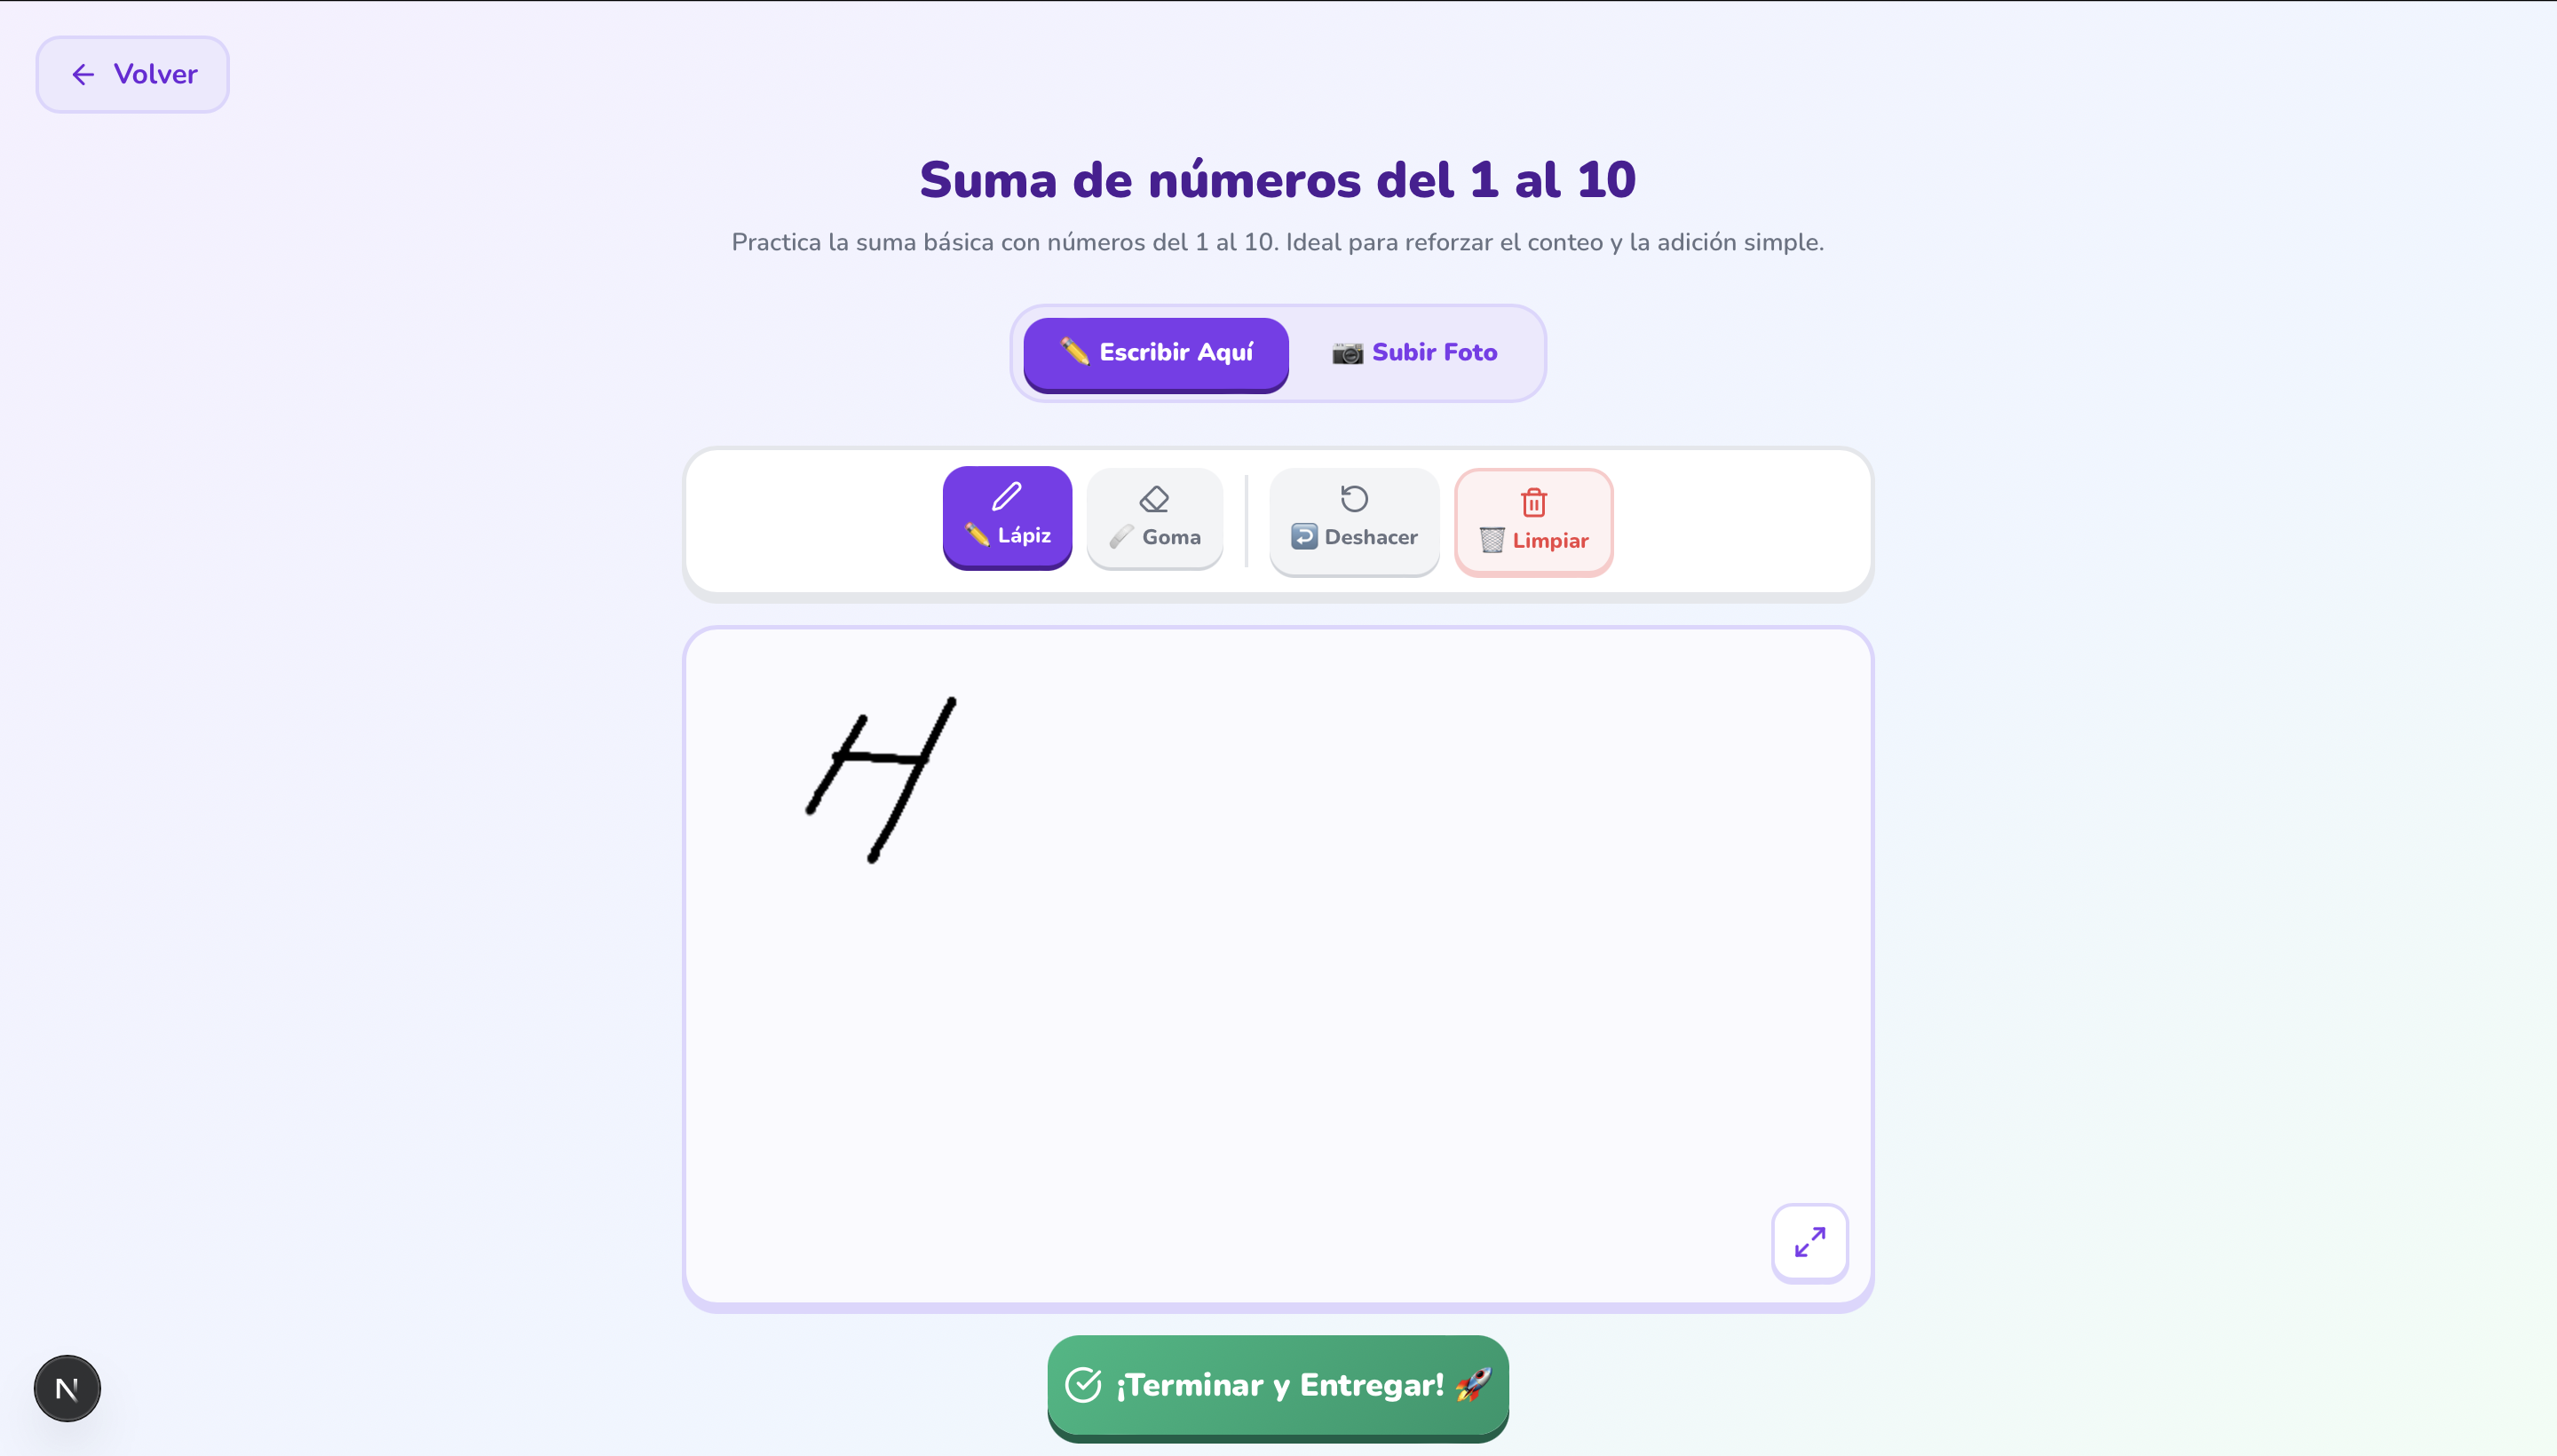
\includegraphics[width=0.7\textwidth]{Imagenes/lienzo.png}
    \caption{Visualización del lienzo digital para realizar ejercicios de escritura}
    \label{fig:lienzo}
\end{figure}


\subsubsection{Vista de captura de escritura}

\begin{figure}[H]
    \centering
    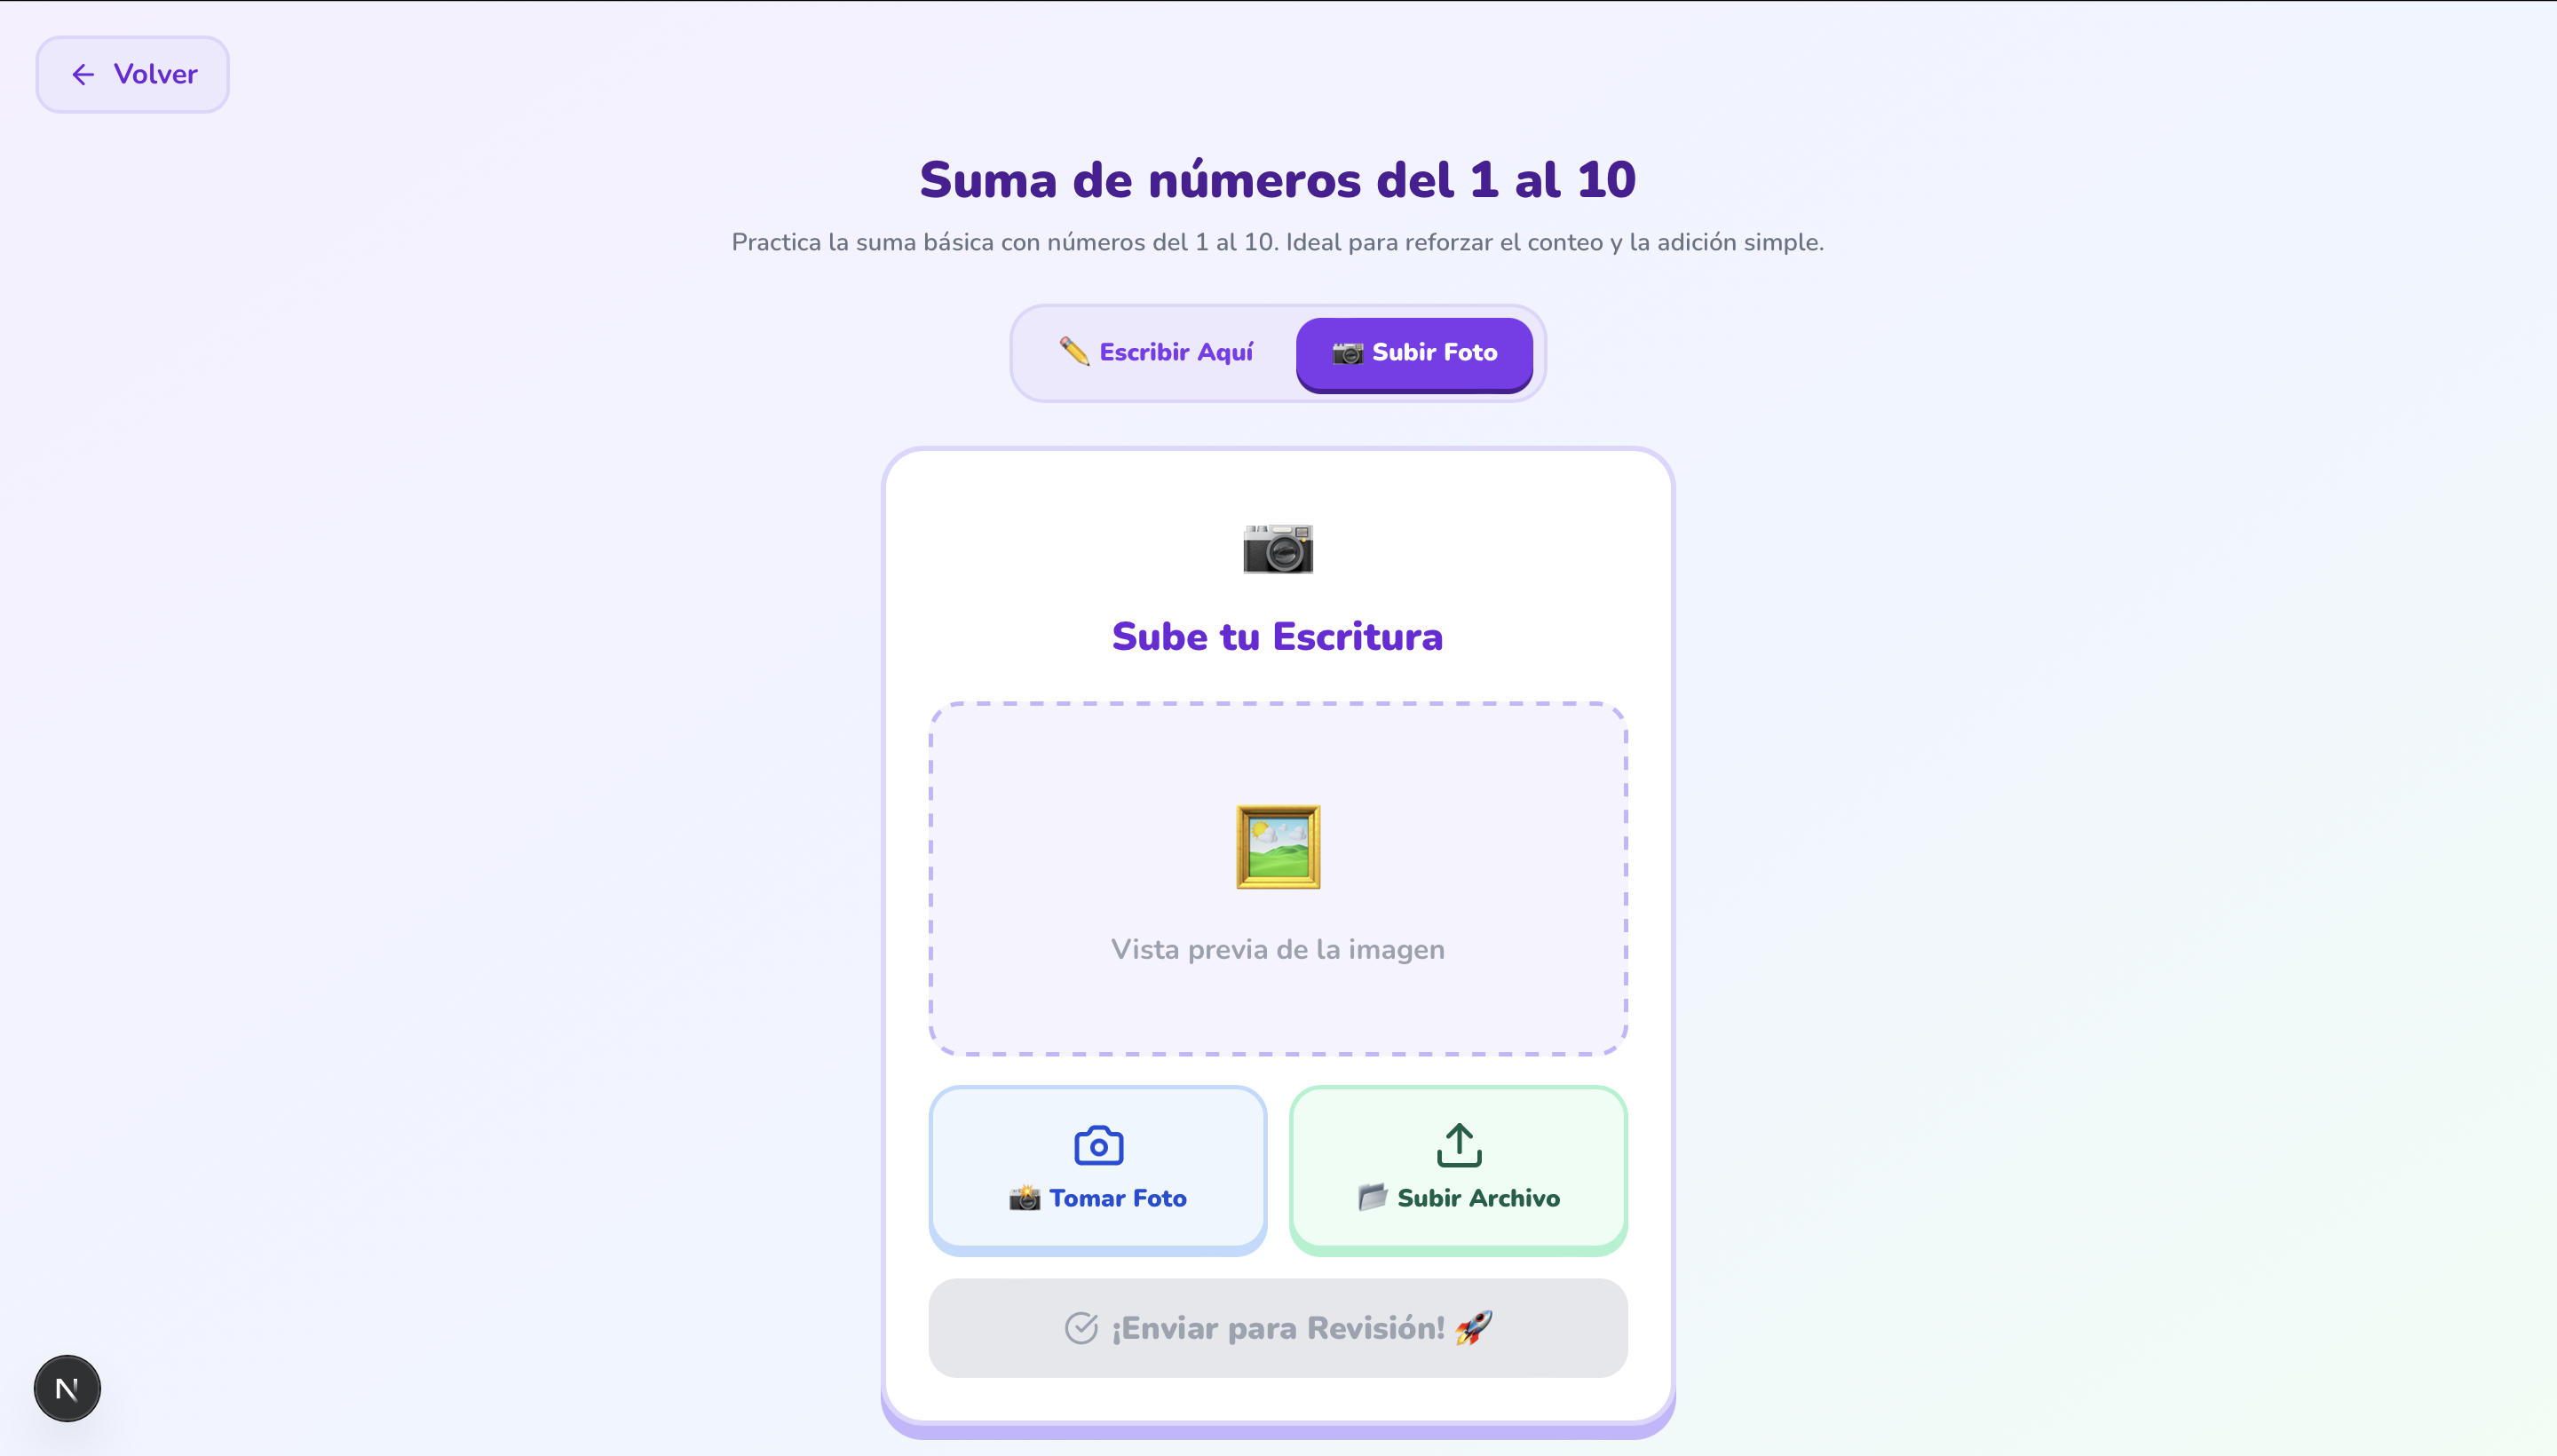
\includegraphics[width=0.7\textwidth]{Imagenes/subirArchivo.png}
    \caption{Visualización de carga de imagen para registrar ejercicios mediante fotografía o archivo}
    \label{fig:subirArchivo}
\end{figure}

\subsubsection{Vista de resultados y retroalimentación}

\begin{figure}[H]
    \centering
    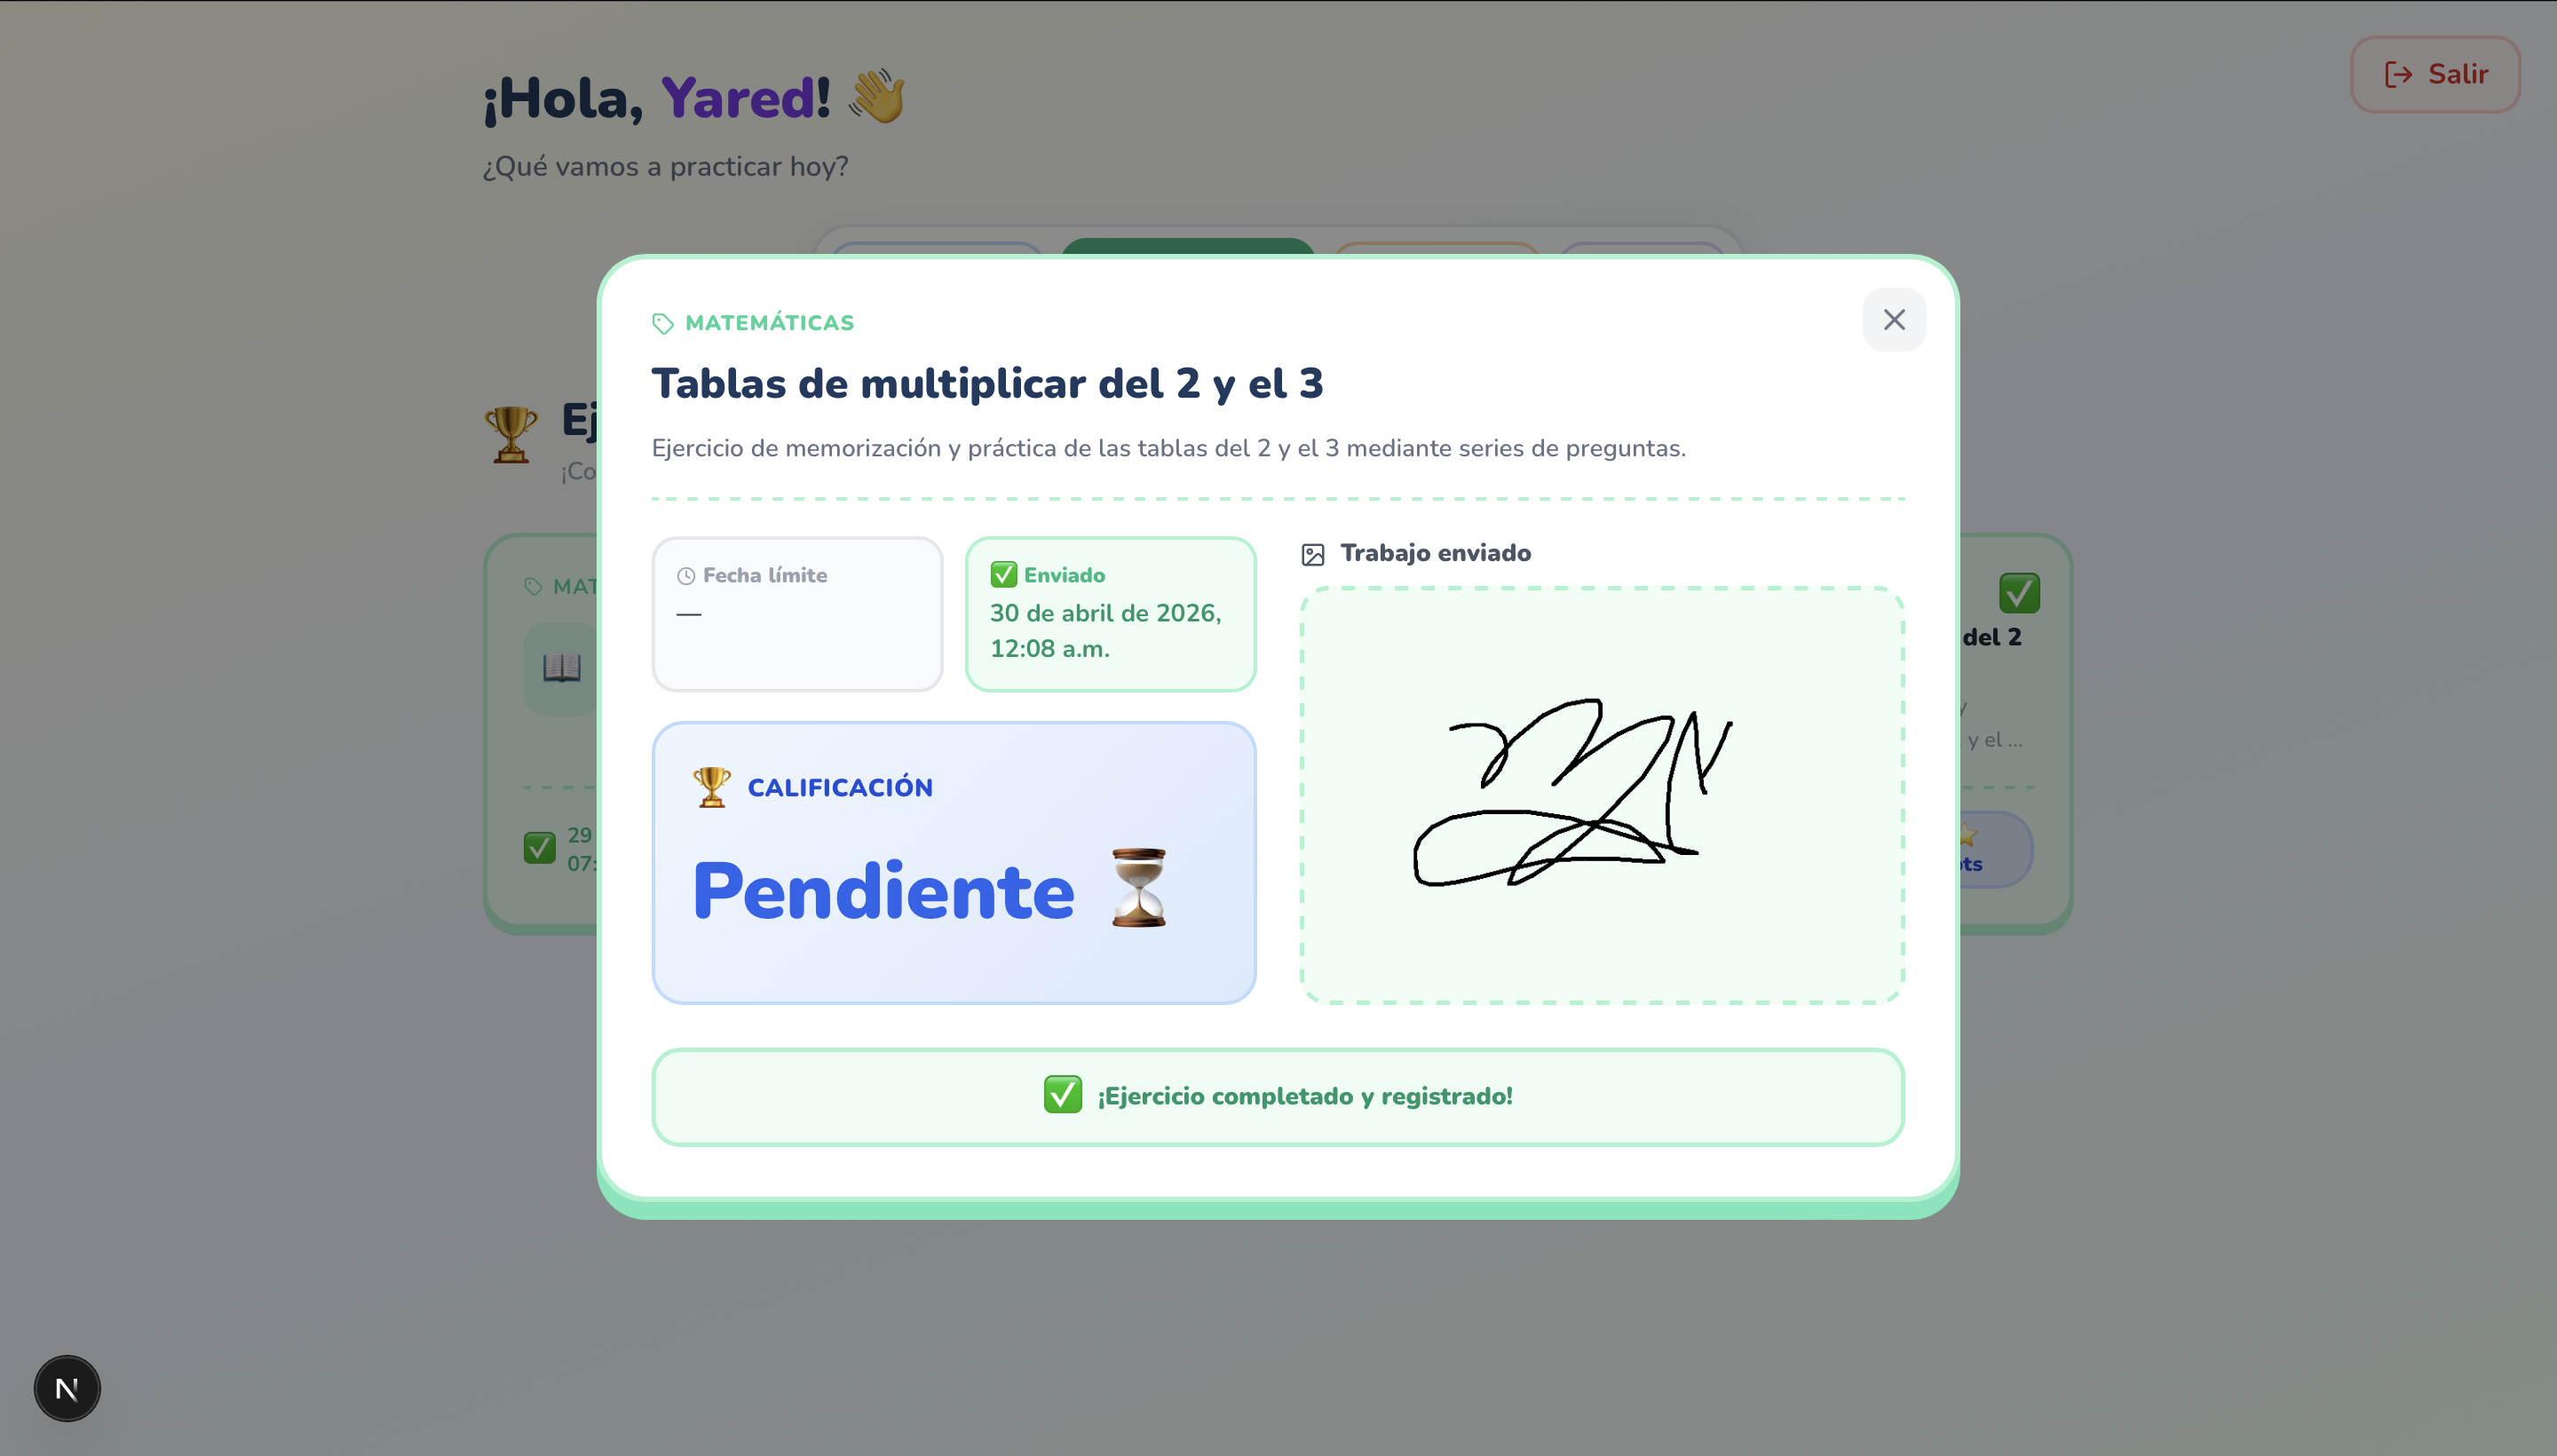
\includegraphics[width=0.7\textwidth]{Imagenes/resultadosEje.png}
    \caption{Visualización de resultados y retroalimentación de ejercicios realizados}
    \label{fig:resultadosEje}
\end{figure}